%% thesis.tex 
%% 

\documentclass[12pt]{article}  
\usepackage[margin=1.0in]{geometry}
\usepackage{setspace}
\usepackage{amsmath}
\usepackage{xfrac}
\usepackage[titletoc,toc,title]{appendix}
\usepackage[T1]{fontenc}
\usepackage{times}
\doublespacing
%\usepackage{latexsym} 
%\usepackage{sparticles} 	%Package for displaying sparticle names. 
%\usepackage{feynmf}
%\usepackage{lmodern}
%\usepackage[T1]{fontenc}
%\usepackage{textcomp}
\usepackage{graphicx} 
%\usepackage[hang,small,bf]{caption2}
\usepackage{caption}
\usepackage{subcaption}
\usepackage{cite}

%\title{TITLE OF YOUR LIFE WORK} 

\begin{document} 
\pagestyle{plain}
%\nolofigures

%\centerline{\textbf{Measurement of the Proton Form Factor Ratio $G_E/G_M$  from Double Spin Asymmetries}} 
\begin{center}
\textbf{Proton Form Factor Ratio, ${\mu_p G_E^p/G_M^p}$ from Double Spin Asymmetry} 
\end{center}

{
\raggedleft
\underline{\textbf{Abstract}}
}

The form factors are fundamental properties of the nucleon representing the effect of its structure on its response to electromagnetic probes such as electrons. The ratio of the electric and magnetic form factors of the proton has been measured for elastic electron-proton scattering up to $Q^2=5.66$ (GeV/c)$^2$ using the double spin asymmetry for target spin orientation aligned perpendicular to the beam momentum direction. 
%They are functions of the four-momentum transfer squared $Q^2$ between the electron and the proton. 
%The form factors, $G_E$ and $G_M$ are experimentally accessible through \emph{Rosenbluth separation method} and \emph{double-polarization observables}. Both methods are sensitive to the form factors in different ways. There are two classes of double-polarization observables, the \emph{polarization-transfer method} and the \emph{double spin asymmetry} which has the same sensitivity to the form factor ratio as the first class. polarization-transfer method offer superior sensitivity to the electric form factor at higher $Q^2$. However, double spin asymmetry experiments were not carried out as the Rosenbluth or polarization-transfer experiments. 
%This paper reports the results of a new measurement of the ratio of the electric and magnetic form factors of the proton up to $Q^2=5.66$ (GeV/c)$^2$ using the double spin asymmetry with a polarized beam and target.

%Experiment E07-003 (SANE, Spin Asymmetries of the Nucleon Experiment) was carried out in Hall C at Jefferson Lab in 2009 to study the proton spin structure functions with a dynamically polarized ammonia target and longitudinally polarized electron beam. By detecting elastically scattered protons in the High-Momentum Spectrometer (HMS) in coincidence with the electrons in the Big Electron Telescope Array (BETA), elastic measurements were carried out in parallel. The elastic double spin asymmetry allows one to extract the proton electric to magnetic form factor ratio $G_E^p/G_M^p$ at high-momentum transfer, $Q^2=5.66$ (GeV/c)$^2$. In addition to the coincidence data, inclusively scattered electrons from the polarized ammonia target were detected by HMS, which allows to measure the beam-target asymmetry in the elastic region with the target spin nearly perpendicular to the momentum transfer, and to extract $G_E^p/G_M^p$ at low $Q^2=2.06$ (GeV/c)$^2$. 

This alternative measurement of $G_E^p/G_M^p$ has verified and confirmed the dramatic discrepancy at high $Q^2$ between the Rosenbluth and the recoil-polarization-transfer method with a different measurement technique and systematic uncertainties uncorrelated to those of the recoil-polarization measurements. The measurement of the form factor ratio at $Q^2=2.06$ (GeV/c)$^2$ has been determined as $\mu_p G_E^p/G_M^p=0.605\pm0.178_{stat}\pm0.033_{sys}$ which is in agreement with an earlier measurement with the polarized target technique at similar kinematics. The same measurement at $Q^2=5.66$ (GeV/c)$^2$ has been determined as $\mu_p G_E^p/G_M^p=0.672\pm0.362_{stat}$ which represents the highest $Q^2$ reach with the double spin asymmetry to date.

{
\raggedleft
\underline{\textbf{I Introduction}}
}

Detailed knowledge of the nucleon is very important to understand the nucleus. Electron scattering is the best tool to probe deep inside nucleons and nuclei. In the one-photon exchange (Born) approximation, the structure of the nucleon is characterized by the electric and magnetic (Sachs) form factors $G_E (Q^2 )$ and $G_M (Q^2 )$, which depend only on the four-momentum transfer squared, $Q^2$. 

The Rosenbluth separation technique has been the first method to separate the proton form factors $G_E^p$ and $G_M^p$ by measuring the elastic electron scattering cross sections at different angles and energies and fixed $Q^2$. In addition, the proton $G_E^p/G_M^p$ ratio has been extracted from measurements of recoil polarization components. By taking the ratio of polarization components, which is proportional to $G_E^p/G_M^p$, many of the systematic errors of the experiment are canceled. 

Measurement of the beam-target asymmetry using double polarization experiments with polarized target is a third technique to extract $G_E^p/G_M^p$ which has not been conducted as often as Rosenbluth separation or recoil polarization experiments. For elastic scattering of polarized electrons from a polarized target, the beam-target asymmetry, $A_p$ is directly related to the proton elastic form factor ratio, $G_E^p/G_M^p$ as;
 \begin{equation}
 \begin{aligned}
\label{btasym}
A_p=\frac{-br\sin \theta^* \cos \phi^*-a\cos \theta^* }{r^2+c},
 \end{aligned}
 \end{equation}
where $r=G_E^p/G_M^p$. The polar and azimuthal angles, $\theta^*$ and $\phi^*$ describe the orientation of the polarization vector relative to $q$, where the $y$ axis points perpendicular to the scattering plane defined by the electron three-momenta ($\vec{p_e} \times \vec{p_{e'}}$). The quantities $a,b,c$ are kinematic factors given by,
 \begin{equation}
 \begin{aligned}
\label{btasymabc}
&a=2 \tau \tan \frac{\theta_e}{2}\sqrt{1+\tau+(1+\tau)^2\tan^2 \frac{\theta_e}{2}}\\
&b=2 \tan \frac{\theta_e}{2}\sqrt{\tau(1+\tau)}\\
&c=\tau+2\tau(1+\tau)\tan^2\frac{\theta_e}{2}
\end{aligned}
\end{equation}
with $\tau=\frac{Q^2}{4M^2}$. 

where $\theta_e$ is the electron scattering angle.
%\begin {equation}
%\begin {aligned}
%\label {asym}
%A_p=\frac{-br\sin\theta^*\cos\phi^*-a\cos\theta^*}{r^2+c}
%\end {aligned}
%\end {equation}
%is directly related to the form factor  ratio, $r=G_E^p/G_M^p$. The polar and azimuthal angles, $\theta^*$ and $\phi^*$ describe the orientation of the polarization vector relative to $q$, where the $y$ axis points perpendicular to the scattering plane defined by the electron three-momenta ($\vec{p_e} \times \vec{p_{e'}}$). The quantities $a,b,c$ are kinematic factors given by $a=2\tau\tan\frac{\theta_e}{2}\sqrt{1+\tau+(1+\tau)^2\tan^2\frac{\theta_e}{2}}$, $b=2\tan\frac{\theta_e}{2}\sqrt{\tau(1+\tau)}$ and $c=\tau+2\tau(1+\tau)\tan^2\frac{\theta_e}{2}$ with $\tau= Q^2/\mid4M^2\mid$ and where $\theta_e$ is the electron scattering angle.


\begin{figure}[htbp]
\centering
\mbox{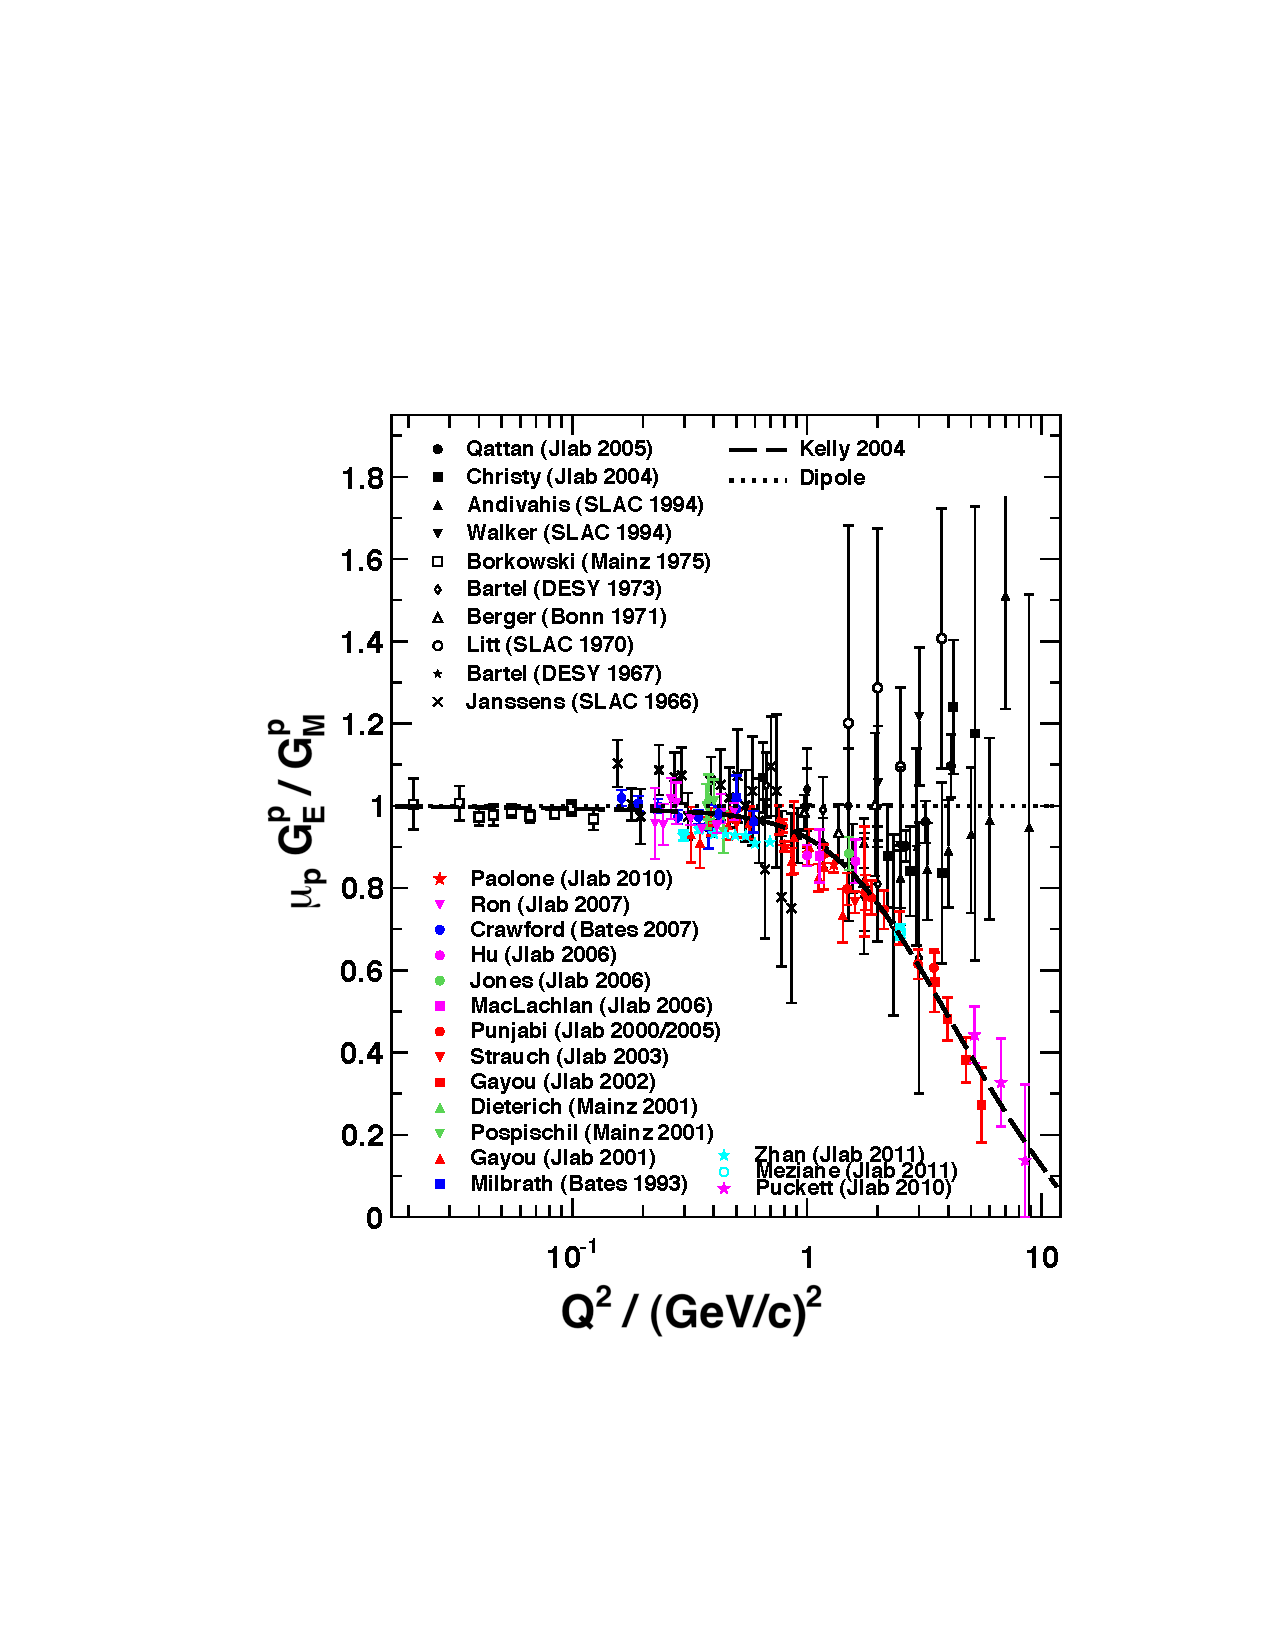
\includegraphics[scale=0.5]{gepgmp}}
\caption{Proton electric to magnetic form factor ratio from Rosenbluth-separated cross-sections (\emph{black symbols}) \cite{26, 27, 28, 29, 30, 31, 32, 33, 34, 35} and from double-polarization experiments (colored symbols) \cite{43, 44, 45, 46, 47, 48, 49, 50, 51, 52, 53, 54, 55, 56, 57, 58, 59, 60}. Theoretical model by Kelly \cite{99} is also shown.}
\label{fig1}
\end{figure}

The world data of the proton form factor ratio $\mu_pG^p_E/G^p_M (\mu_p=2.79)$ from the Rosenbluth-separated method \cite{26, 27, 28, 29, 30, 31, 32, 33, 34, 35}  are shown in Figure \ref{fig1} along with those obtained from the double polarization experiments with recoil polarization  \cite{43, 44, 45, 46, 47, 48, 49, 50, 51, 52, 53, 54, 55, 56, 57, 58} and polarized target \cite{59,60}. A linear fall-off of the polarization data can be seen compared to the nearly flat $Q^2$ dependence of $G_E^p/G_M^p$ measured with the Rosenbluth technique. One possible solution that explains the difference between the two experimental methods is two-photon exchange (TPE) \cite{89, 90, 91, 92, 93, 94, 95, 96, 97, 98}.

Having the same sensitivity as the recoil polarization technique to the TPE effects, the third technique,  beam-target asymmetry is a good way to verify the systematic errors in the recoil polarization technique. By measuring $G_E^p/G_M^p$ and comparing it to the previous results, the discovery of any unknown or underestimated systematic errors in the previous measurements is possible. The first such measurement was done by the experiment RSS at Jefferson Lab at $Q^2=1.5$ $(GeV/c)^2$ \cite{60}. Carrying out the same measurement at higher $Q^2$ values is very important to study the consistency of the third technique, double-spin asymmetry with the first two techniques, Rosenbluth separation and recoil polarization. In this work, the polarized target method is applied at $Q^2 = 2.20$, $5.17$, and $6.25$ $(GeV/c)^2$ as a by-product of the experiment SANE.
% (\textbf{S}pin \textbf{A}symmetries of the \textbf{N}ucleon \textbf{E}xperiment) conducted in Hall C at Jefferson Lab in 2009. 

Section II presents the description of the experimental setup. Section III presents the detailed description of the data analysis method, including the elastic event selection, raw/physics asymmetry calculation, extraction of the proton form factor ratio, $\mu_pG^p_E/G^p_M$, and estimation of the systematic uncertainties. Section IV presents the final results of the experiment and discuss the impact of the measurement on the world database of proton electromagnetic form factor ratio. An overview of the theoretical uncertainty of the nucleon electromagnetic form factors is also discussed. Section V presents the conclusion. 

\vspace{8 mm}

{
\raggedleft
\underline{\textbf{II Experimental Setup}}
}

The experiment E07-003 (Spin Asymmetries of the Nucleon Experiment) is a single-arm inclusive-scattering experiment. The goal of SANE was to measure proton spin structure functions $g_1(x, Q^2)$ and $g_2(x, Q^2)$ at four-momentum transfer $2.5\textless Q^2 \textless 6.5$ (GeV/c)$^2$ and $0.3 \textless x \textless 0.8$ which is an extension of the kinematics of experiment RSS \cite{179} performed in Hall C, Jefferson Lab in 2007. 
 

SANE measured the inclusive spin asymmetries with the target spin aligned parallel and nearly perpendicular (80$^{\circ}$) to the beam direction for longitudinally polarized electron scattering from a DNP polarized proton (crystallized NH$_3$) target. The experiment was carried out in the experimental Hall C at Jefferson Lab from January to March, 2009. A subset of the data was used to measure the elastic beam-target spin asymmetry from elastic electron-proton scattering. Polarized electrons with energies 4.72 GeV and 5.89 GeV were scattered from the polarized proton target with the spin of the proton aligned nearly perpendicular (80$^{\circ}$) to the beam direction. 
Recoiled protons were detected by the High-Momentum Spectrometer (HMS) at $22.3^{\circ}$ and $22.0^{\circ}$, and central momenta of 3.58 $GeV/c$ and 4.17 $GeV/c$, respectively, for the two different beam energies. Scattered electrons were detected by the Big Electron Telescope Array (BETA) in coincidence with the proton in HMS. 
In addition to that, single-arm electron scattering data were also taken by detecting the elastically scattered electron in the HMS at a central angle of $15.4^{\circ}$ and 4.4 $GeV/c$ HMS central momentum for an electron beam energy of 5.89 GeV.

The Continuous Electron Beam Accelerator Facility (CEBAF) at the Thomas Jefferson National Accelerator Facility delivers longitudinally polarized electron beam with $\sim100$ \% duty factor simultaneously to all three experimental halls. This delivers an 85\% polarized electron beam with quantum efficiency of 1\%. More information about the CEBAF accelerator can be found in \cite{100}.
%Polarized electrons are emitted by illuminating Gallium Arsenide (GaAs) cathode using a circularly polarized laser light with a frequency equal to the energy of the band gap of the material. Jefferson Lab's polarized source uses a superlattice GaAs photocathode, in which the pure GaAs is doped by phosphorous, which delivers an 85\% polarized electron beam with quantum efficiency of 1\%.  The orientation of the beam polarization is rotated by a Wien filter before injection into the accelerator to optimize the delivery of longitiudinal polarization to the experimental halls. The photo-emitted electrons are accelerated upto 67 MeV by the injector before entering to the CEBAF linacs. The electron acceleration takes place in superconducting RF-resonant Niobium cavities cooled by super fluid Helium at $\simeq$2 K, giving the maximum energy of approximately 6 GeV. More information about the CEBAF accelerator can be found in \cite{100}.

%The beam is rastered to increase its spot size, which spreads the heat load over a wider area of the target. 
The fast-raster system with a uniform square beam spot of $1\times1$ mm$^2$ \cite{101, 102}, 25 meters upstream of the target is designed to increase the effective beam size in order to prevent damage to the targets due to the high current. 
%The Hall C Beam Position Monitors (BPMs) monitor the beam position continously \cite{103}. 
The Hall C arc dipole magnets are used as a spectrometer to measure the energy of the electron beam as it enters the Hall. Using the curvature of the beam over its 34.4$^{\circ}$ deflection by dipoles and the precise knowledge of the arc dipole fields, the energy of the beam is determined with an accuracy of$\Delta E/E\sim 10^{-4}$. The beam polarization was measured by Hall C M$\phi$ller polarimeter \cite{104}.

In addition to the standard Hall C beam-line equipment, SANE required extra beam-line equipment to accommodate the UVa polarized target. The slow-raster was added to spread the beam over an even larger area of the target material cup. This second raster was circular, with a diameter of 2 cm \cite{105}. Because the raster system rapidly changes the actual beam position on the target during the experiment, SANE used the relative position to the beam center by recording the raster X and Y amplitudes in an ADC. When the target magnetic field is nearly perpendicular to the beam, the electron beam is deflected down, away from the target center. To counteract this, the beam was sent through a chicane of magnets which bent it down and then back up at the target so that it does not miss the center of the target. Even after the beam passed through the target center, it would continue to bend down, deflecting away from the standard beam dump in the Hall. Therefore, an 80-foot-long helium bag was used as an additional beam line from the scattering chamber to the beam dump. The exit windows were large enough to accept the different beam deflections 2.8$^{\circ}$ and 2.2$^{\circ}$ for the different beam energies 4.72 and 5.89 GeV, respectively.

In order to perform a coincidence experiment with the proton detected in HMS, the electron detector is required to have a large acceptance to match the electron acceptance to the proton acceptance defined by the HMS collimator. The lead-glass electromagnetic calorimeter, BigCal, provides the needed acceptance with enough energy and angular resolution \cite{106}.
% It consisted of 1744 type TF1-0 lead-glass bars with an total area of roughly 122$\times$218 cm$^2$. This has a large solid angle of approximately 0.2 Sr with the face of the calorimeter placed 3.50 m from the target cell \cite{106}. 

The primary apparatus for the elastic data is based on the superconducting magnetic spectrometer called High Momentum Spectrometer (HMS), which has a large solid angle and momentum acceptance, providing the capability of analyzing high momentum particles (up to 7.4 GeV/c). This equipped with a set of detectors to detect and track charged particles scattered from the target. In the standard configuration, the HMS consists of a pair of gas drift chambers (DC1 and DC2) \cite{107}, four planes of scintillator hodoscopes (S1X, S1Y, S2X, S2Y) \cite{108}, a gas Cherenkov detector, and a lead-glass calorimeter. The two drift chambers provide the particle tracking information at the focal plane. The scintillator hodoscopes are used for triggering the detector read-out and provide the timing information while the gas Cherenkov detector and the lead-glass calorimeter provide the particle identification. 

As a double polarization experiment, SANE requires a polarized nucleon target. Frozen ammonia (NH${_3}$) was utilized as a polarized proton target. In addition to the polarized target, $^{12}$C and CH$_2$ targets were also used for calibration purposes. The protons in the NH$_3$ molecules were polarized using Dynamic Nuclear Polarization (DNP) in a 5 T magnetic field at 1 K temperature \cite{136}. In DNP, nucleons were polarized by transferring the free electron polarization in the medium to the nucleons. These spin transitions, both electron and nucleon spin flips, are forbidden due to the dipole selection rules. Therefore, these transitions are induced by microwave radiation at high magnetic field and low temperature. 
%In order to form the free, unpaired electrons to use in DNP, ammonia beads were ionized to knock out an atomic hydrogen from NH$_3$ molecules to form $dot{N}$H$_2$ paramagnetic centers. 
The spin direction of the polarized proton can be aligned parallel (positive polarization) or anti-parallel (negative polarization) to the field direction by changing the induced transition frequency applied by microwave radiation. Data were taken at both frequencies. 
%Because of the strong interaction with the lattice, the electrons reach thermal equilibrium very rapidly (in 10$^{-3}$ S) by relaxation to the lowest energy state, allowing it to flip the spin of another proton. However, due to the weak coupling to the lattice, the relaxation time of the nucleons is much larger, $\sim$10$^3$ S. In this way, both positive and negative polarizations can be achieved with the same magnetic field by altering the microwave frequency. 
The positive polarization was reached by applying the microwave radiation with a frequency of 140.1 GHz, while the negative polarization was reached by 140.5 GHz. A Nuclear Magnetic Resonance (NMR) system was used to monitor the polarization of the SANE target \cite{109}.

%Choosing $^{14}$NH$_3$ as the polarizable proton target material has several advantages compared to lithium hydride ($^7$LiH and $^6$LiH) which is the other commonly used irradiation doping DNP target material. Its higher maximum achievable polarization (\textgreater 90 \% at 1 K and 5 T), the high rate at which it reaches the maximum polarization (\textless 30 minutes), its higher resistance to radiation damage caused by an experimental beam and the high percentage of polarizable nucleons for scatterings, its dilution factor, which is roughly 17.6\% protons fpr $^{14}$NH$_3$, are the crucial properties.

SANE used the University of Virginia polarized target. This replaced the standard Hall C target housing called \emph{scattering chamber}. It consisted of a superconducting Helmholtz pair of magnets, a target insert, a liquid helium evaporation refrigerator system and a NMR system.
The superconducting Helmholtz pair of magnets provided 5 T magnetic field to the target. It can rotated around the target so that to change the target field direction. The target insert was roughly 2 m long ladder which provided the room for four target materials, in 2.5 cm diameter target cups. The liquid helium evaporation refrigerator system kept the target material at 1 K temperature and the NMR system provided an online target polarization and recorded the operating conditions. 
The beam-target asymmetry, $A_p$ shown in the Equation \eqref{btasym} is maximum at the proton spin aligned perpendicular to the beam direction. However, due to the constraint on rotating the target superconducting coils, The maximum spin direction one could reach was 80$^{\circ}$ without blocking the BETA acceptance.

The microwave horns were trained on each NH$_3$ target cup to provide the microwave radiation required for target DNP, and the NMR coils were embedded into the two NH$_3$ target cups to measure the target polarizations. Microwave were provided by the Extended Interaction Oscillator (EIO). 

\vspace{8 mm}
{
\raggedleft
\underline{\textbf{Data Analysis}}
}

The determination of the particle trajectory and momentum at the target was done mainly by two major steps. The first step was to find the trajectory, the positions and the angles, $X_{fp}$ and $X'_{fp}$ ($Y_{fp}$ and $Y'_{fp}$) in the dispersive (non-dispersive) direction at the detector focal plane using the two HMS drift chambers. The second step was to reconstruct the trajectory back to the interaction vertex using an HMS optics matrix. Because the optics matrix takes into account the vertical position of the beam at the target, the calculation of momentum and out-of-plane angle are sensitive to the vertical position. The HMS optics matrix has been determined without the target magnetic field. therefore, an additional particle transport through the target magnetic field has been added to the existing HMS particle-tracking algorithm to take account the extra particle deflections due to the target magnetic field. Standard calibrations for all of the HMS detectors have performed \cite{110}.

%First, the particle tracks are reconstructed by the HMS reconstruction coefficients to the target center, assuming no target magnetic field. Then, by knowing the target coordinates, the particle is projected back to the field-free region at z=100 cm from the target center and then transported back to the target center through the target magnetic field, determining new tracked vertical position. If the difference between this tracked vertical position at the target center and the vertical position of the beam measured by the slow-raster is larger than 1 mm, then a new effective vertical position is assumed and the procedure is iterated until the difference between the tracked and measured vertical position is less than 1 mm. Standard calibrations for all of the HMS detectors have performed \cite{110}.

There are a large number of $\pi^0$ events produced in the target. These neutral pions decay very rapidly into two photons. The BigCal calibration was done using the energy deposited in two separated clusters in BigCal from these two neutral photons.

{
\raggedleft
\underline{\textbf{Elastic Event Selection}}
}

Identification of electrons in HMS was done with PID and momentum acceptance cuts. By using the Cherenkov cut, the number of photoelectrons on the Cherenkov counter $\textgreater 2$ and the calorimeter cut, $E_{cal}/P\textgreater0.7$, (PID cuts), the backgrounds due to $\pi^-$ particles were suppressed. The quantities, $E_{cal}$ is the deposited energy in the HMS calorimeter. The HMS spectrometer measured the momentum of the detected electron, P.

\begin{figure}[htbp]
\centering
        \begin{subfigure}[htbp]{0.45\textwidth}
               \centering
               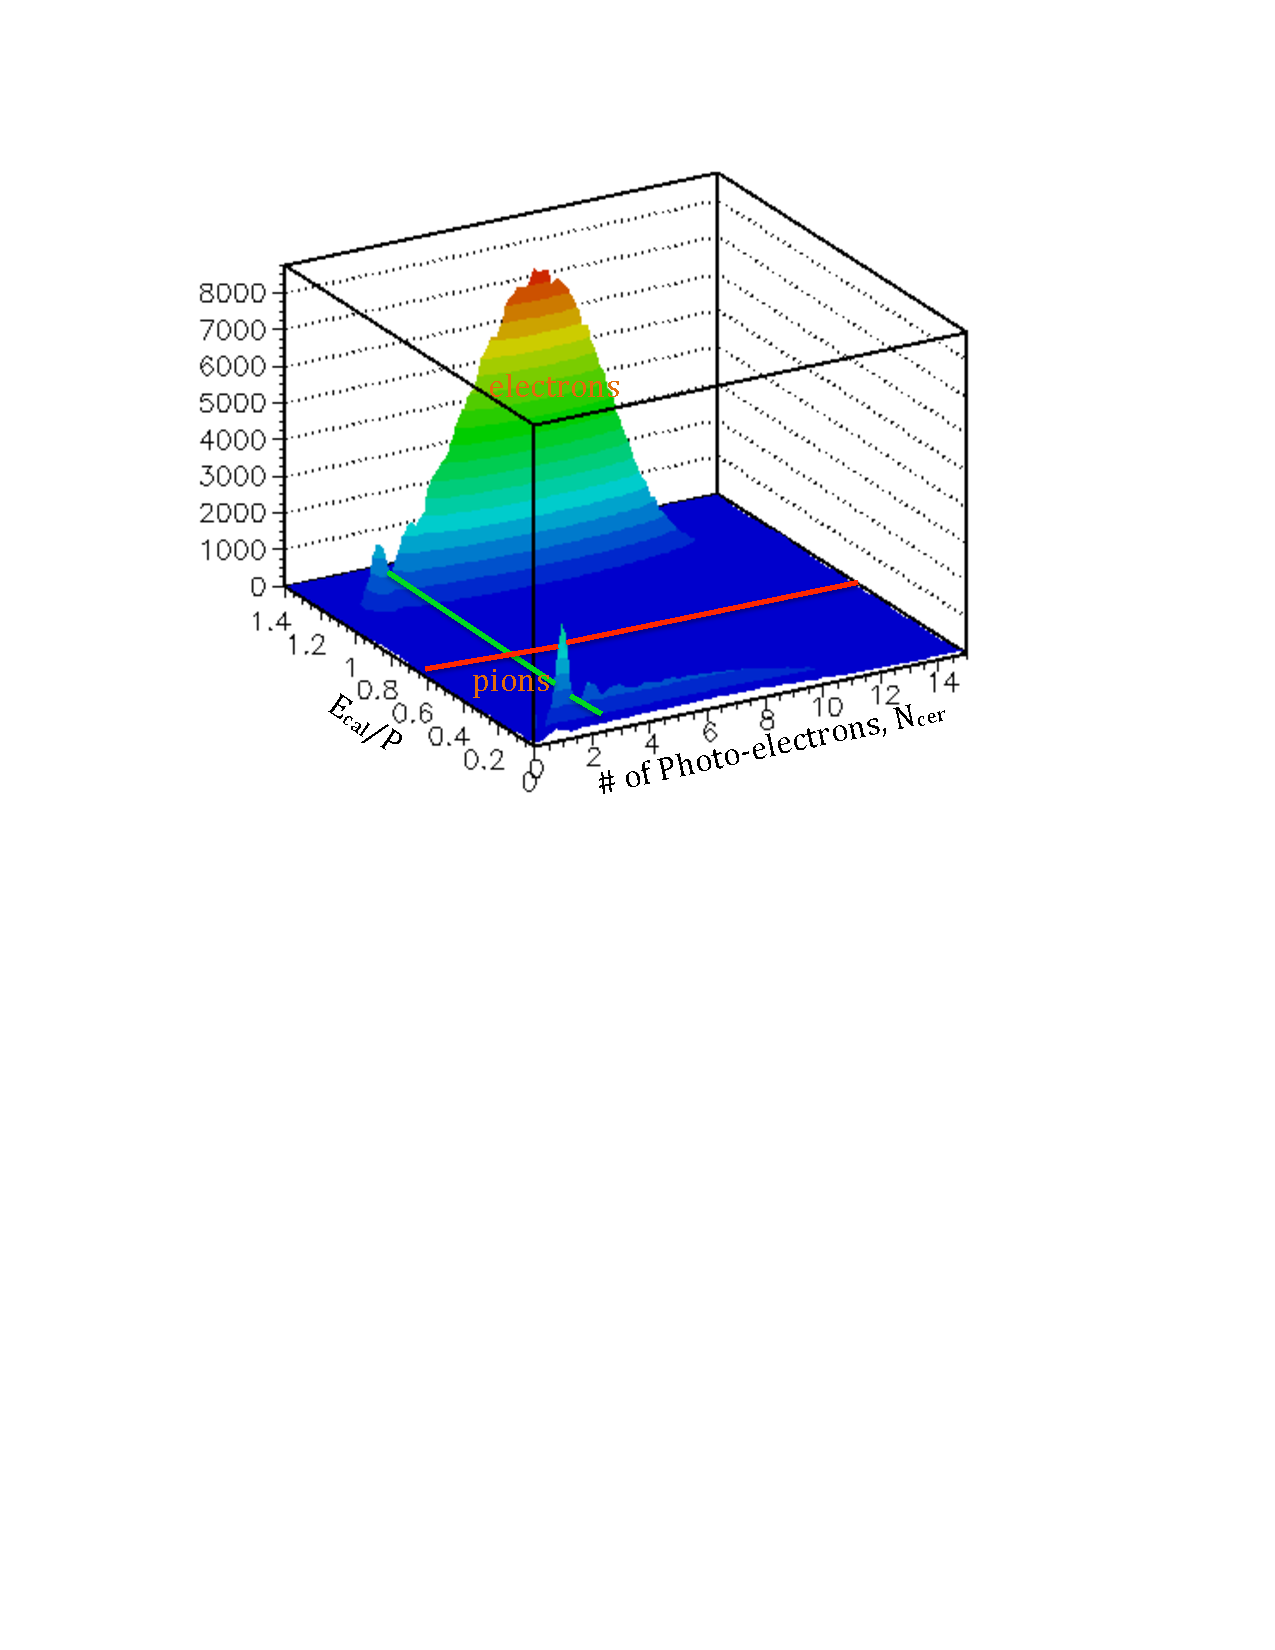
\includegraphics[width=\textwidth]{cer_calo}
                \label{dctime_72994}
      \end{subfigure}
          \begin{subfigure}[htbp]{0.20\textwidth}
                \centering
               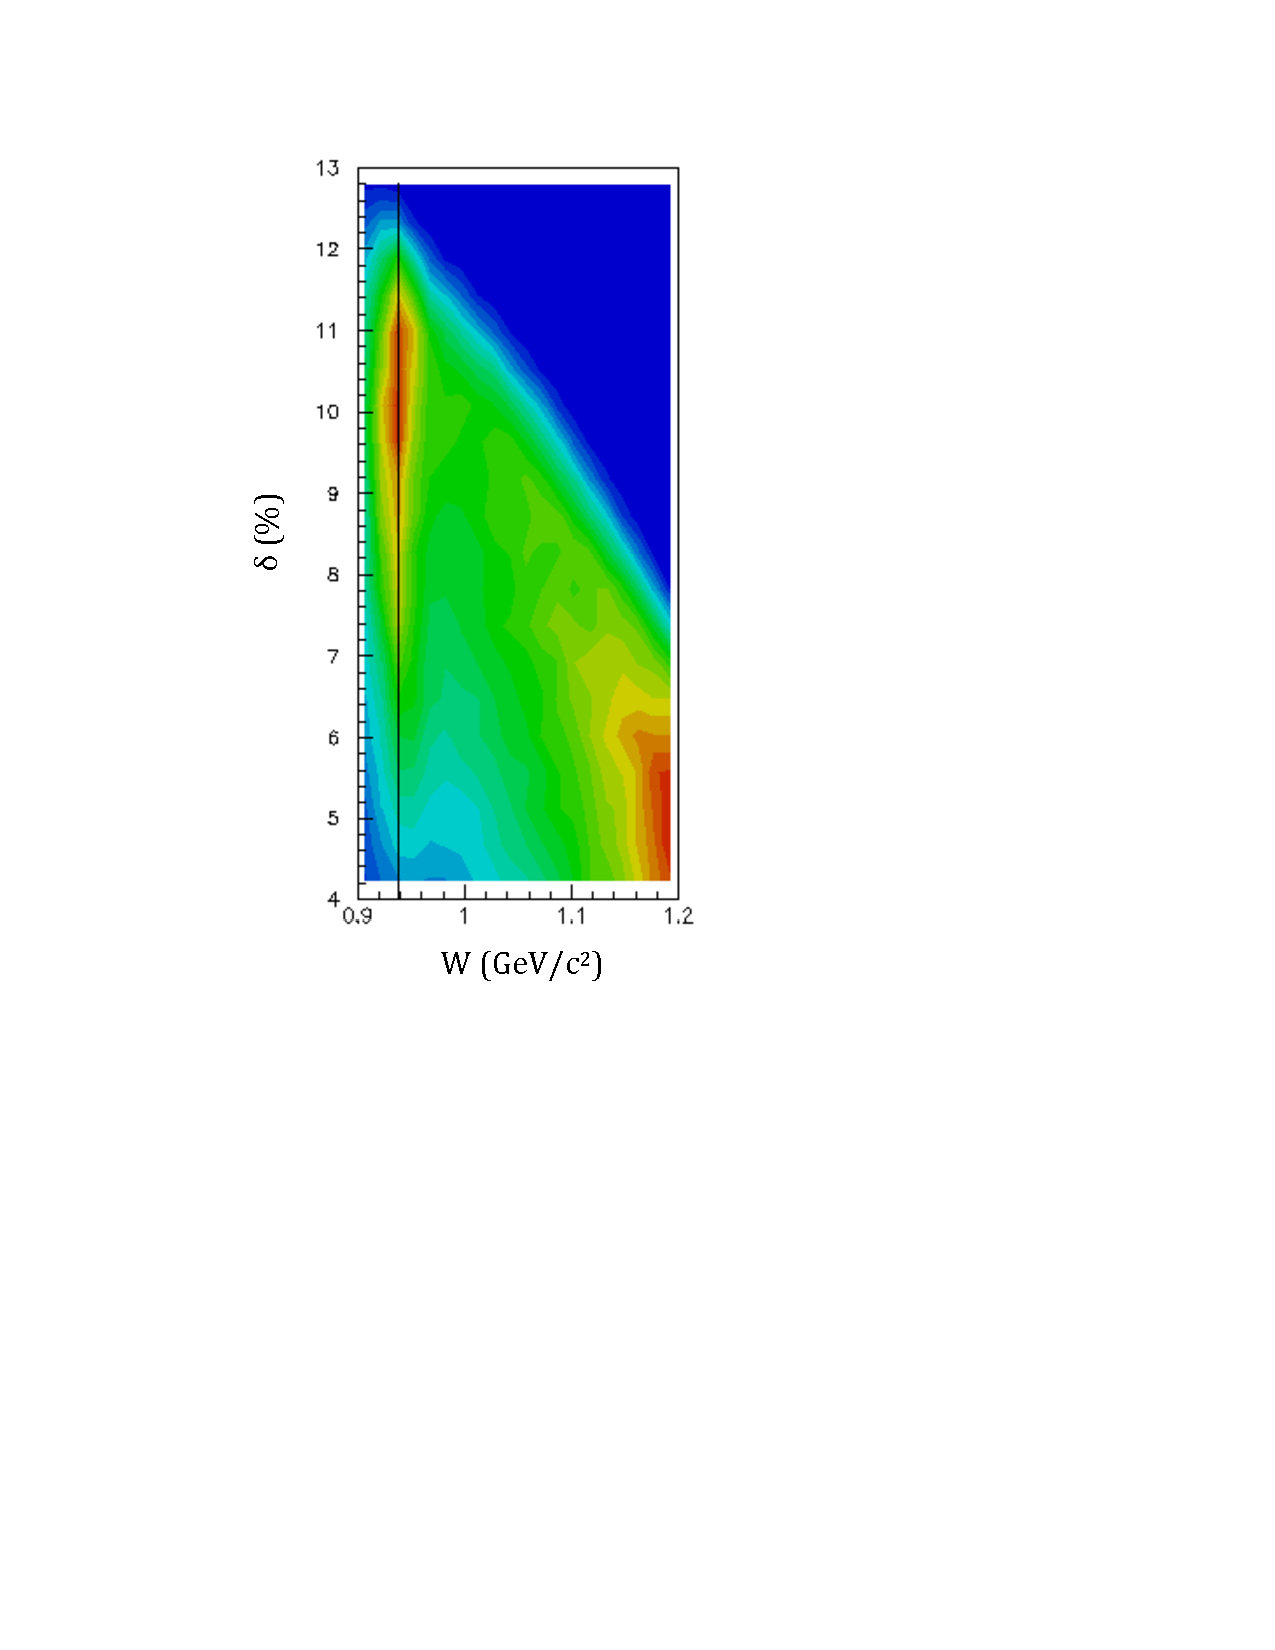
\includegraphics[width=\textwidth]{delta}
                \label{dc_dist}
        \end{subfigure}    
\vspace{-0.4cm}         
\caption{\emph{Left}: Cherenkov photo electrons and calorimeter energy regions for both pions and electrons. The red (green) line indicates the calorimeter (Cherenkov) cut which was used to separate electrons. \emph{Right}: The momentum acceptance of the total single-arm electron data as a function of invariant mass.}
\label{dccalib}                  
\end{figure}

An acceptance cut on the relative momentum, $\delta = \frac{P-P_c}{P_c}=\frac{\delta P}{P}$, which is well determined for the region $-8\%\textless \delta \textless 10\%$ has been applied to the data in addition to the PID cuts. $P_c$ is the central momentum of HMS. This eliminates events that are outside of the spectrometer acceptance, but end up in the detectors after multiple scattering in the magnets or exit windows. Because the elastic events were mostly populated in the higher region of the $\delta$ acceptance, $10\% \textless \delta \textless 12\%$, where the reconstruction matrix elements are not well known, these data were analyzed separately so that the systematic uncertainty from the HMS optics can be determined separately. Therefore, two $\delta$ intervals of the elastic data, $-8\% \textless \delta \textless 10\%$ and $10\% \textless \delta \textless 12\%$, were used separately in addition to the PID cuts to extract the elastic events.  Using this higher $\delta$ region of $10\% \textless \delta \textless 12\%$, about $\sim40\%$ of extra events were gained. 

%The extraction of the elastics events from the coincidence data have been done using both HMS and BigCal quantities. By knowing the incoming electron beam energy, E and by measuring the recoil proton angle, $\theta_p$ in HMS, the horizontal (vertical) coordinate X (Y) of the scattered electron at the lead-glass calorimeter (BigCal) in BETA was measured, and also calculated from the elastic kinematics on the proton (HMS). An elliptic cut on $\Delta Y = (Y_{HMS}-Y_{BETA})$ vs $\Delta X = (X_{HMS}-X_{BETA})$,

The extraction of the elastics events from the coincidence data have been done using both HMS and BigCal quantities. 
The horizontal (vertical) coordinate X (Y) of the scattered electron at the lead-glass calorimeter (BigCal) in BETA was measured, and also calculated from the elastic kinematics of the proton in HMS by knowing the incoming electron beam energy, E and the recoil proton angle, $\theta_p$. An elliptic cut of $\Delta Y = (Y_{HMS}-Y_{BETA})$ vs $\Delta X = (X_{HMS}-X_{BETA})$,
\[
\sqrt{\left(\frac{\Delta X}{X_{cut}}\right)^2+\left(\frac{\Delta Y}{Y_{cut}}\right)^2} \le 1. \]
reduced the background most effectively than using the cuts of $\Delta X$ and $\Delta Y$ separately, because the shape of the cut matches the shape of the elastic peak in two dimensional phase space, ($\Delta X, \Delta Y$). Here, ($X_{cut}, Y_{cut}$)=(7, 10) cm.

Based on energy and momentum conservation for electron-proton elastic scattering, the relative momentum difference, $\Delta_p=\frac{P-P_p(\theta_p)}{P_c}\times 100$ between the proton momentum measured by HMS, P and the momentum predicted by the scattered proton angle, $P_p$, using Equation \eqref{pp}, 
\begin{equation}
\label{pp}
P_p(\theta_p)=\frac{2M_pE(E+M_p)\cos {\theta_p}}{M_p^2+2M_pE+E^2\sin^2{\theta_p}},
\end{equation}
which is expressed as a percentage of the HMS central momentum, $P_c$ is defined. The width of the $\Delta_p$ cut was chosen to be $\pm 3 \sigma \simeq \pm 0.02$ and applied for further background suppression for the coincidence data.
\begin{figure}[htbp]
\centering
        \begin{subfigure}[htbp]{0.49\textwidth}
               \centering
               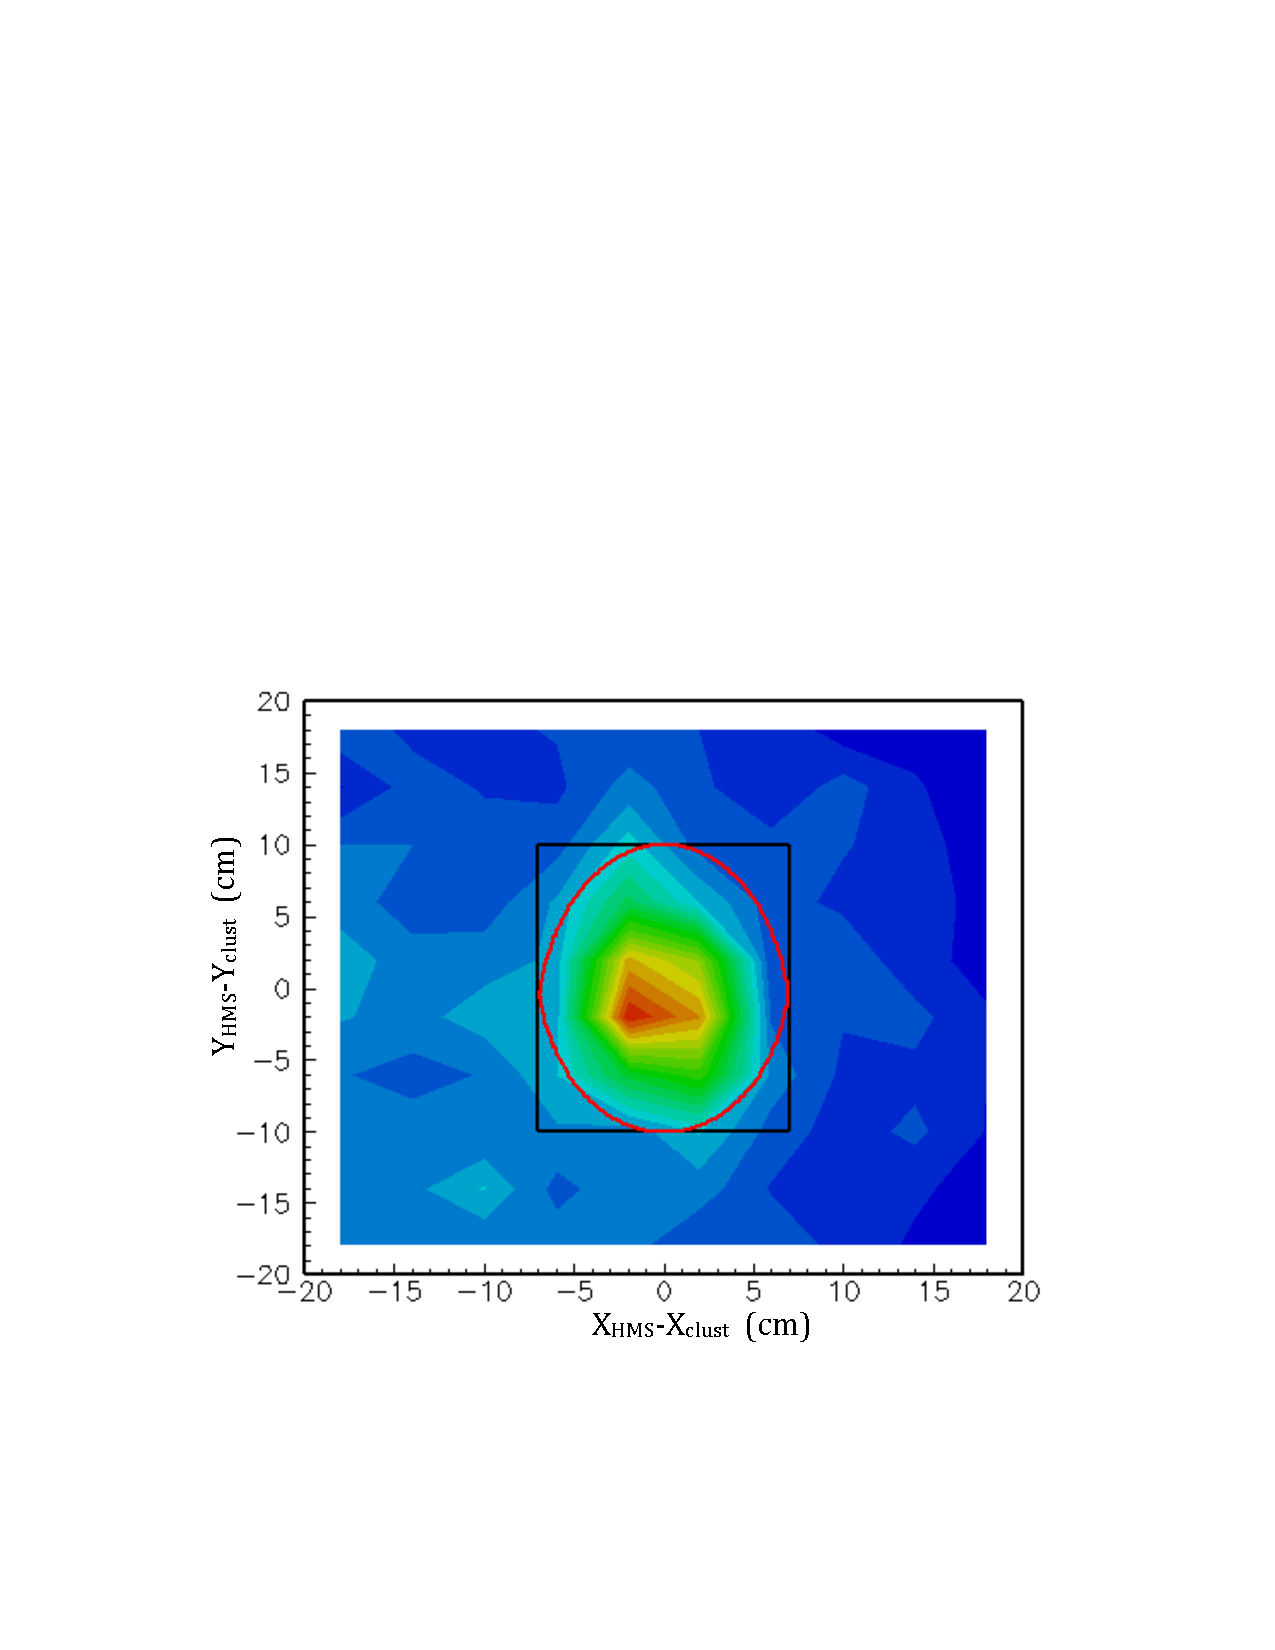
\includegraphics[width=\textwidth]{xydiff5}
                \label{xdiff}
      \end{subfigure}
          \begin{subfigure}[htbp]{0.49\textwidth}
                \centering
               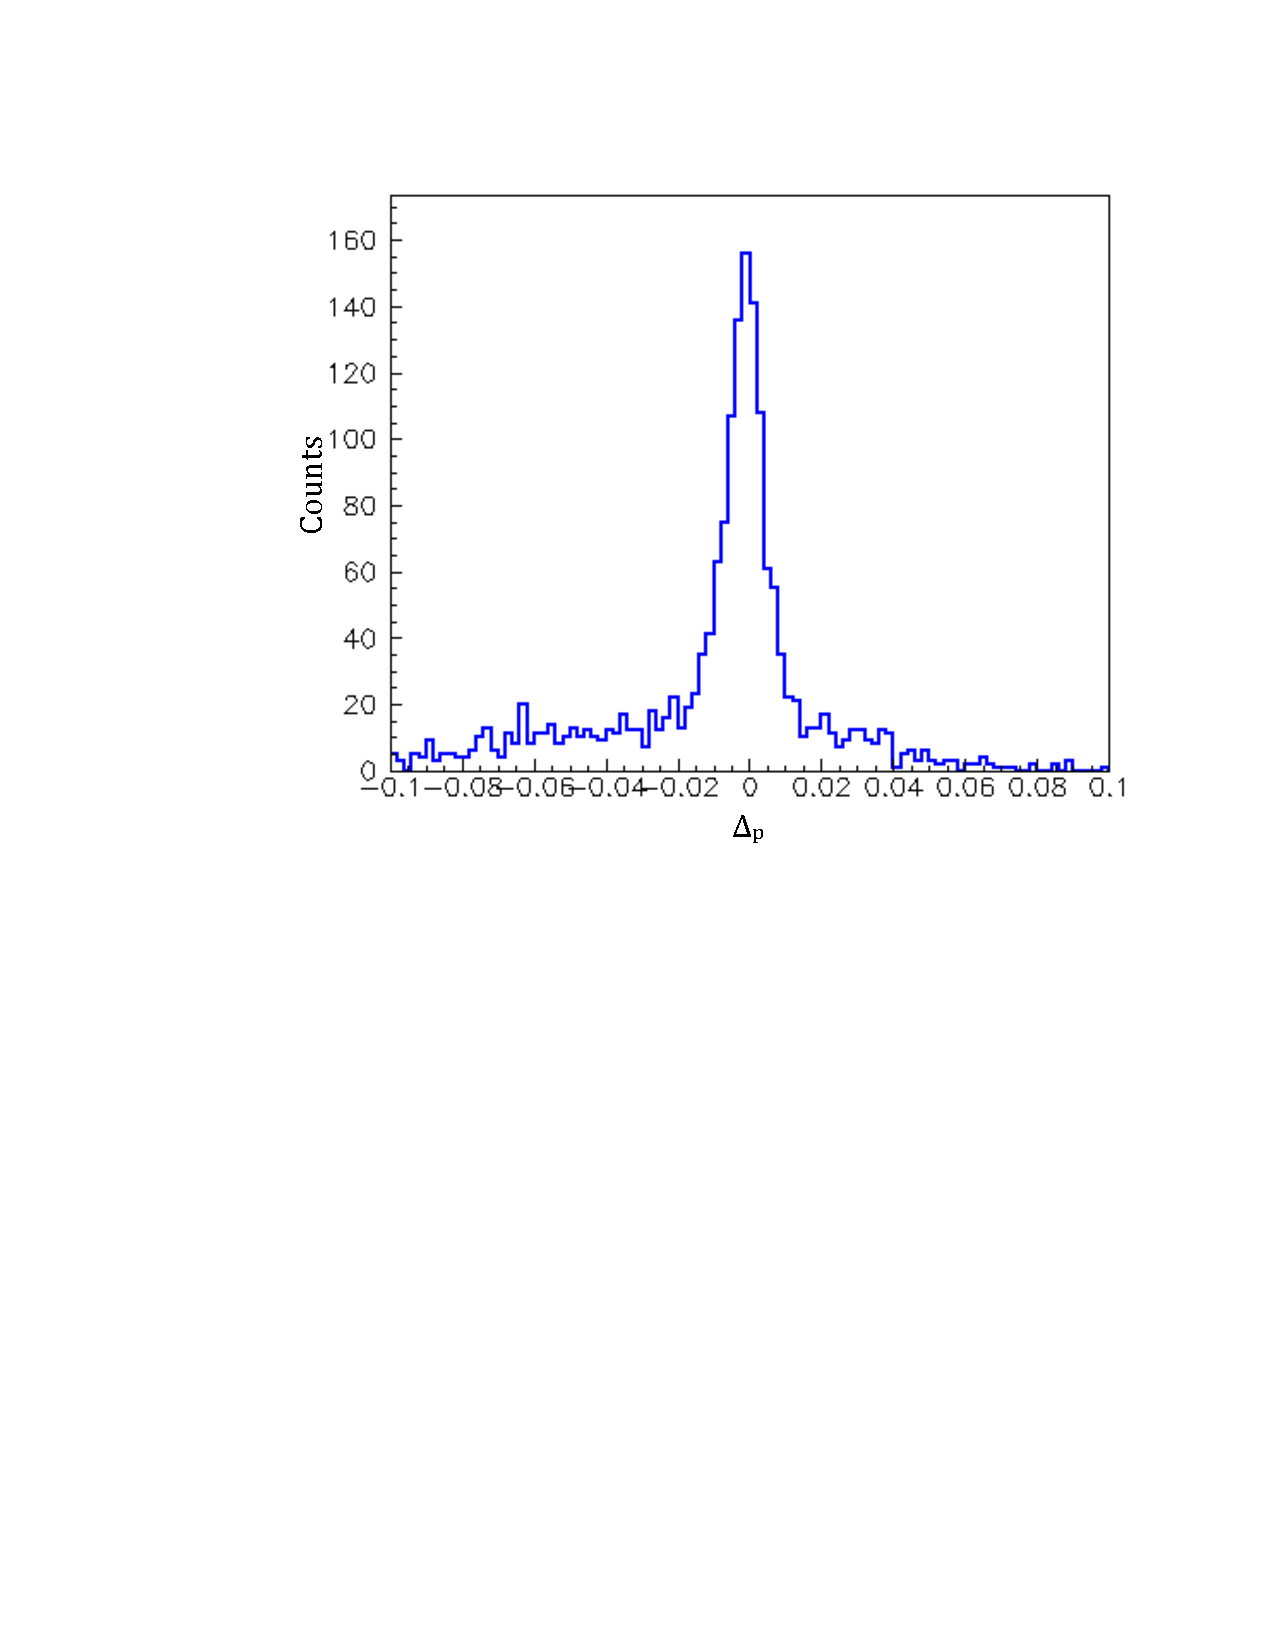
\includegraphics[width=\textwidth]{dp_cut5}
                \label{ydiff}
        \end{subfigure}    
        
\caption{\emph{Left}: The elliptical cut (red) with $(X_{cut},Y_{cut})=(7,10)$ $cm$ applied to the $\Delta Y$ vs $\Delta X$ spectra at $Q^2=6.26$ (GeV/c)$^2$. \emph{Right}: The $\Delta_p$ spectra of all events after applying the elliptical cut at $Q^2=6.26$ (GeV/c)$^2$.}
\label{xydiff}                  
\end{figure}

The beam and target offsets were determined on data using data-to-Monte Carlo simulation comparison for both single-arm and coincidence data. For the single-arm data, the invariant mass, W had a slight dependence on the out-of-plane angle at the target. In addition, For the coincidence data, $\Delta_p$ $(Y_{BETA})$ had a dependence on the out-of-plane angle at the target ($\Delta Y$). An azimuthal angle dependence was added to the target field map used in the calculation of the electron track that changed the electron's reconstructed momentum and hence the reconstructed vertical position, which eliminated the above dependencies. 

{
\raggedleft
\underline{\textbf{Raw/ Physics Asymmetries}}
}

The measured asymmetries on the extracted elastic events were formed by,
%scattering of polarized electrons from a transversely polarized target, the beam-target asymmetry,
\begin {equation}
\begin {aligned}
\label {rasym}
A_r=\frac{N^+-N^-}{N^++N^- } 
\end {aligned}
\end {equation}                            
where,  $N^+$ and $N^-$ were the raw elastic counts normalized by the deadtime-corrected charge for opposite beam helicities. Hence the physics asymmetries,
\begin {equation}
\begin {aligned}
\label {pasym}
A_p=\frac{A_r}{P_B P_Tf} +N_c
\end {aligned}
\end {equation}                 
were obtained by normalizing the measured asymmetries, $A_r$ by target and beam polarizations, $P_T$ and $P_B$, and the dilution factor, $f$\footnote{The dilution factor is the ratio of the yields of scattering off free protons to that from the entire target.}. The $N_c$ term is a correction to the measured asymmetry that eliminates the contribution from quasi-elastic scattering off polarized $^{15}N$ under the elastic peak. Because SANE used $^{14}NH_3$ (ammonia), the correction by $N_c$ for $^{14}N$ was negligible but of opposite sign as for $^{15}N$ \cite{60}.

%The electron single-arm data and the coincidence data were analyzed separately. For the single-arm electron data, after applying a relative momentum acceptance cut of $-8\%$ to $+10\%$ for the HMS spectrometer, and particle identification cuts on the data, elastic events were extracted. By knowing the incoming beam energy, $E$ and measuring the scattered electron angle, $\theta_e$, and scattered electron energy, $E'$ by the HMS spectrometer, the invariant mass, $W$ has been calculated for the extracted elastic event.
% \begin{equation}
%\label{wmass}
%W^2=M^2-Q^2+2M(E-E')
%\end{equation}
%where the four-momentum transfer squared, $Q^2$ is determined as;
% \begin{equation*}
%\label{eq}
%E'=\sfrac{E}{\left[{1+\frac{2E\sin^2{\left({\frac{\theta_e}{2}}\right)}}{M}}\right]}, \,\,\,\,\,\,\,\,\,\,\,\,\,\,\,\,\,\,\,\, 
%Q^2=4EE'\sin^2\left(\frac{\theta_e}{2}\right) 
%\end{equation*}
%using elastic kinematics.

A Monte Carlo simulation was used to estimate the backgrounds and to determine the dilution factor, $f$. The dilution factor only involves materials in the beam, which electrons can scatter off. Assuming $NH_3$ in the liquid $He$ bath\footnote{The target ladder was immersed in a liquid $He$ bath to maintain 1 K temperature, which cooled down from 4 K by pumping off the liquid from the evaporation refrigerator in order to optimize the target polarization.}, $H$, $N$, $He$ and $Al$\footnote{Contributions arised from the target cup lids, the 4 K shield and the refrigerator's tailpiece.} were simulated and compared with the single-arm elastic data. Because two different $NH_3$ target cups have been used with different packing fractions\footnote{The packing fraction is the ratio of the volume taken by the ammonia to the entire target cup volume which was determined by comparing the measured and the simulated yields.}, the dilution factors were determined separately. 
%Figure \ref{mc}(left) shows a comparison of simulated target contributions with the elastic data for the bottom target. 

The dilution factors were calculated for both targets by taking the ratio of the difference between the total raw yields and the Monte Carlo background yields ($N+He+Al$) to the total raw yield.  
\begin{equation}
\label{dfsin}
f=\frac{Yield_{data}-MC_{(N+He+Al)}}{Yield_{data}}.
\end{equation}

The obtained dilution factors are shown in Figure \ref{trg_cont} (right) for top target for two different $\delta$ regions.
\begin{figure}[htbp]
\centering
        \begin{subfigure}[htbp]{0.31\textwidth}
               \centering
               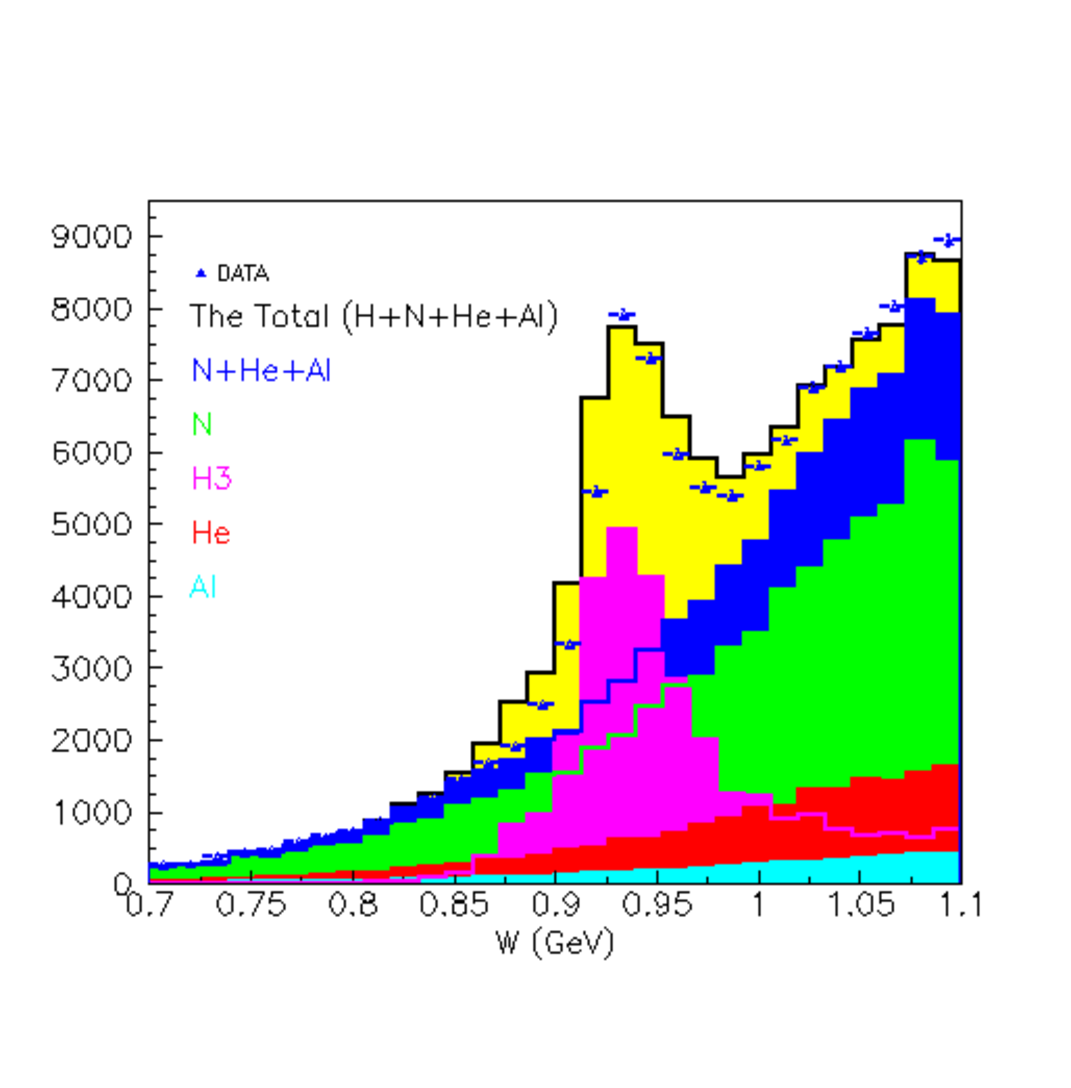
\includegraphics[width=\textwidth]{trg_cont810}
                \label{trg_cont810}
      \end{subfigure}
          \begin{subfigure}[htbp]{0.31\textwidth}
                \centering
               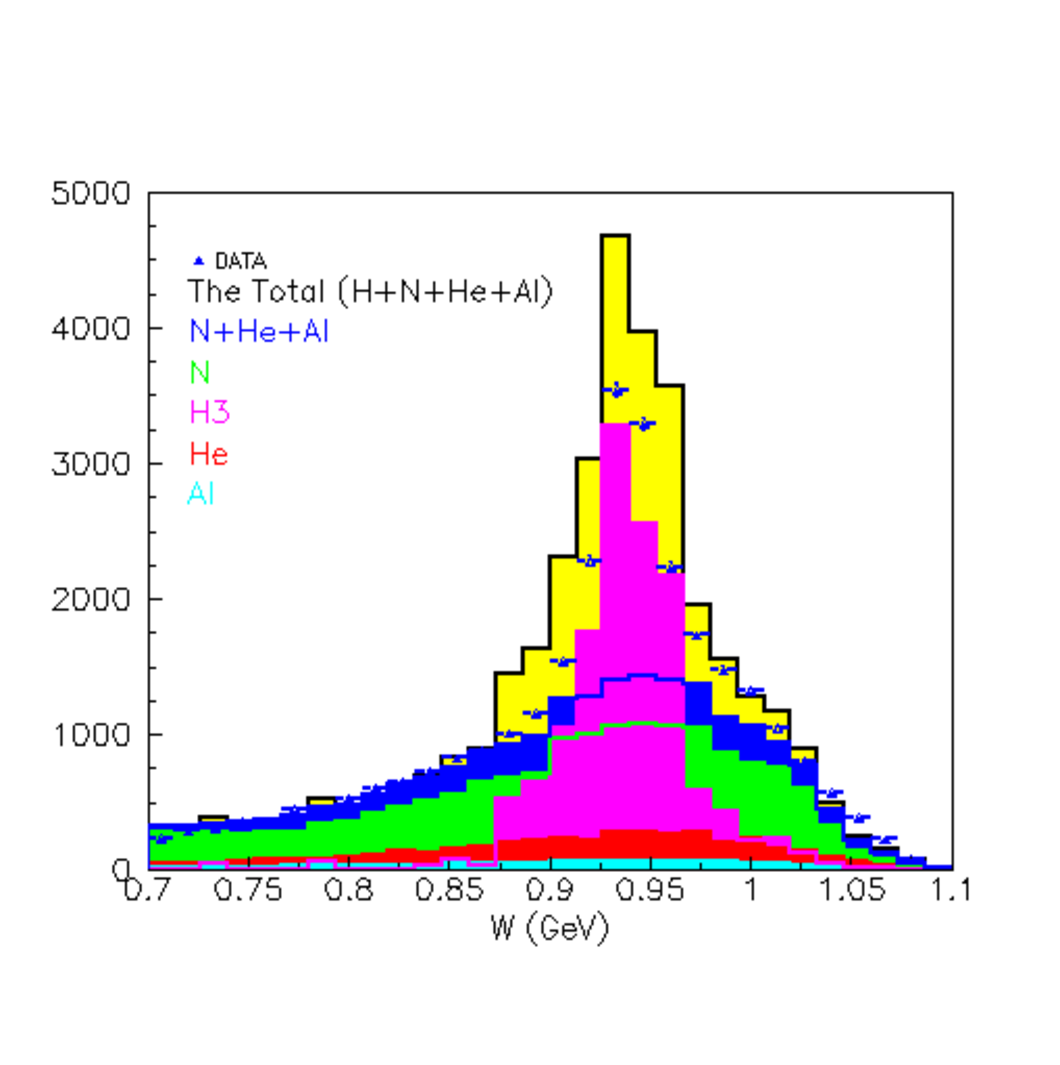
\includegraphics[width=\textwidth]{trg_cont1012}
                \label{trg_cont1012}
        \end{subfigure}   
           \begin{subfigure}[htbp]{0.34\textwidth}
                \centering
               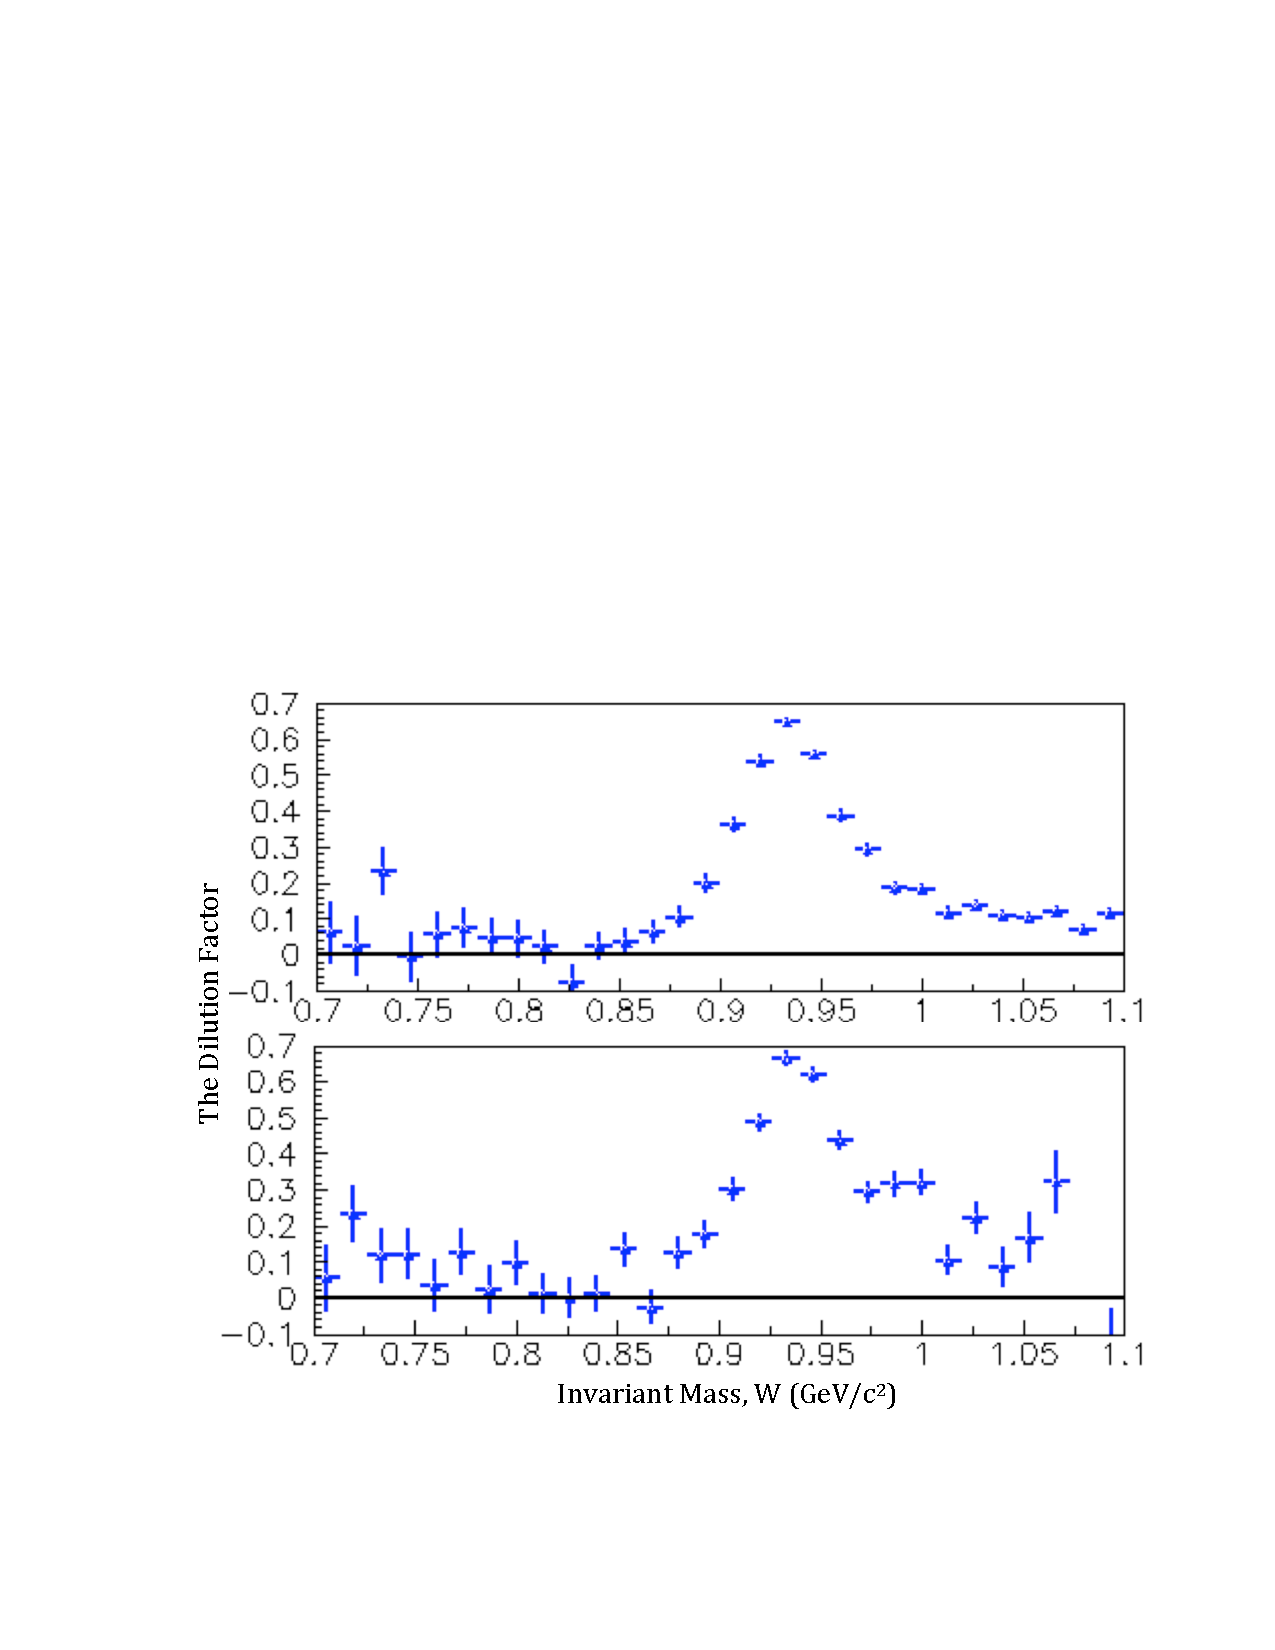
\includegraphics[width=\textwidth]{reldf}
                \label{reldf}
        \end{subfigure}         
\vspace{-0.4cm}         
\caption{The simulated target contributions at the elastic peak compared to the data at both $\delta$ regions,   $-8\% \textless \delta \textless 10\%$ (\emph{left}) and $10\% \textless \delta \textless 12\%$ (\emph{center}) for the top target using experiment run 72795. Different colors show different target type contributions. \emph{Right}: The calculated dilution factors for $-8\% \textless \delta \textless 10\%$ (\emph{top}) and $10\% \textless \delta \textless12\%$ (\emph{bottom}) for the top target using run 72795.}
\label{trg_cont}                  
\end{figure}

The physics asymmetries, $A_p$ and its errors, $\Delta A_p$ were calculated for the extracted elastic events using Equation \eqref{pasym} by using the average values for $P_B=73\% $, $P_T=70\%$, and normalizing with the dilution factor, $f$ for each $W$ bin. The average physics asymmetry and it's error at the elastic reagion were determined for both top and bottom targets by using a linear fit in the region of 0.91\textless W \textless0.97 GeV/c$^2$, where higher dilution factor exists.  
%The physics asymmetries and their errors were determined for both top and bottom targets by using a linear fit in the region of 0.91\textless W \textless0.97 GeV/c$^2$, where the higher dilution factor exists. 

Figure \ref{apsinglearm} (\emph{left}) shows the top and bottom physics asymmetries for the two different $\delta$ regions. The weighted average $A_p$ and $\Delta A_p$ were obtained by combining the top and bottom asymmetries for both $\delta$ regions. The results are shown in Figure \ref{apsinglearm} (\emph{right}) 

\begin{figure}[htbp]
\centering
        \begin{subfigure}[htbp]{0.49\textwidth}
               \centering
               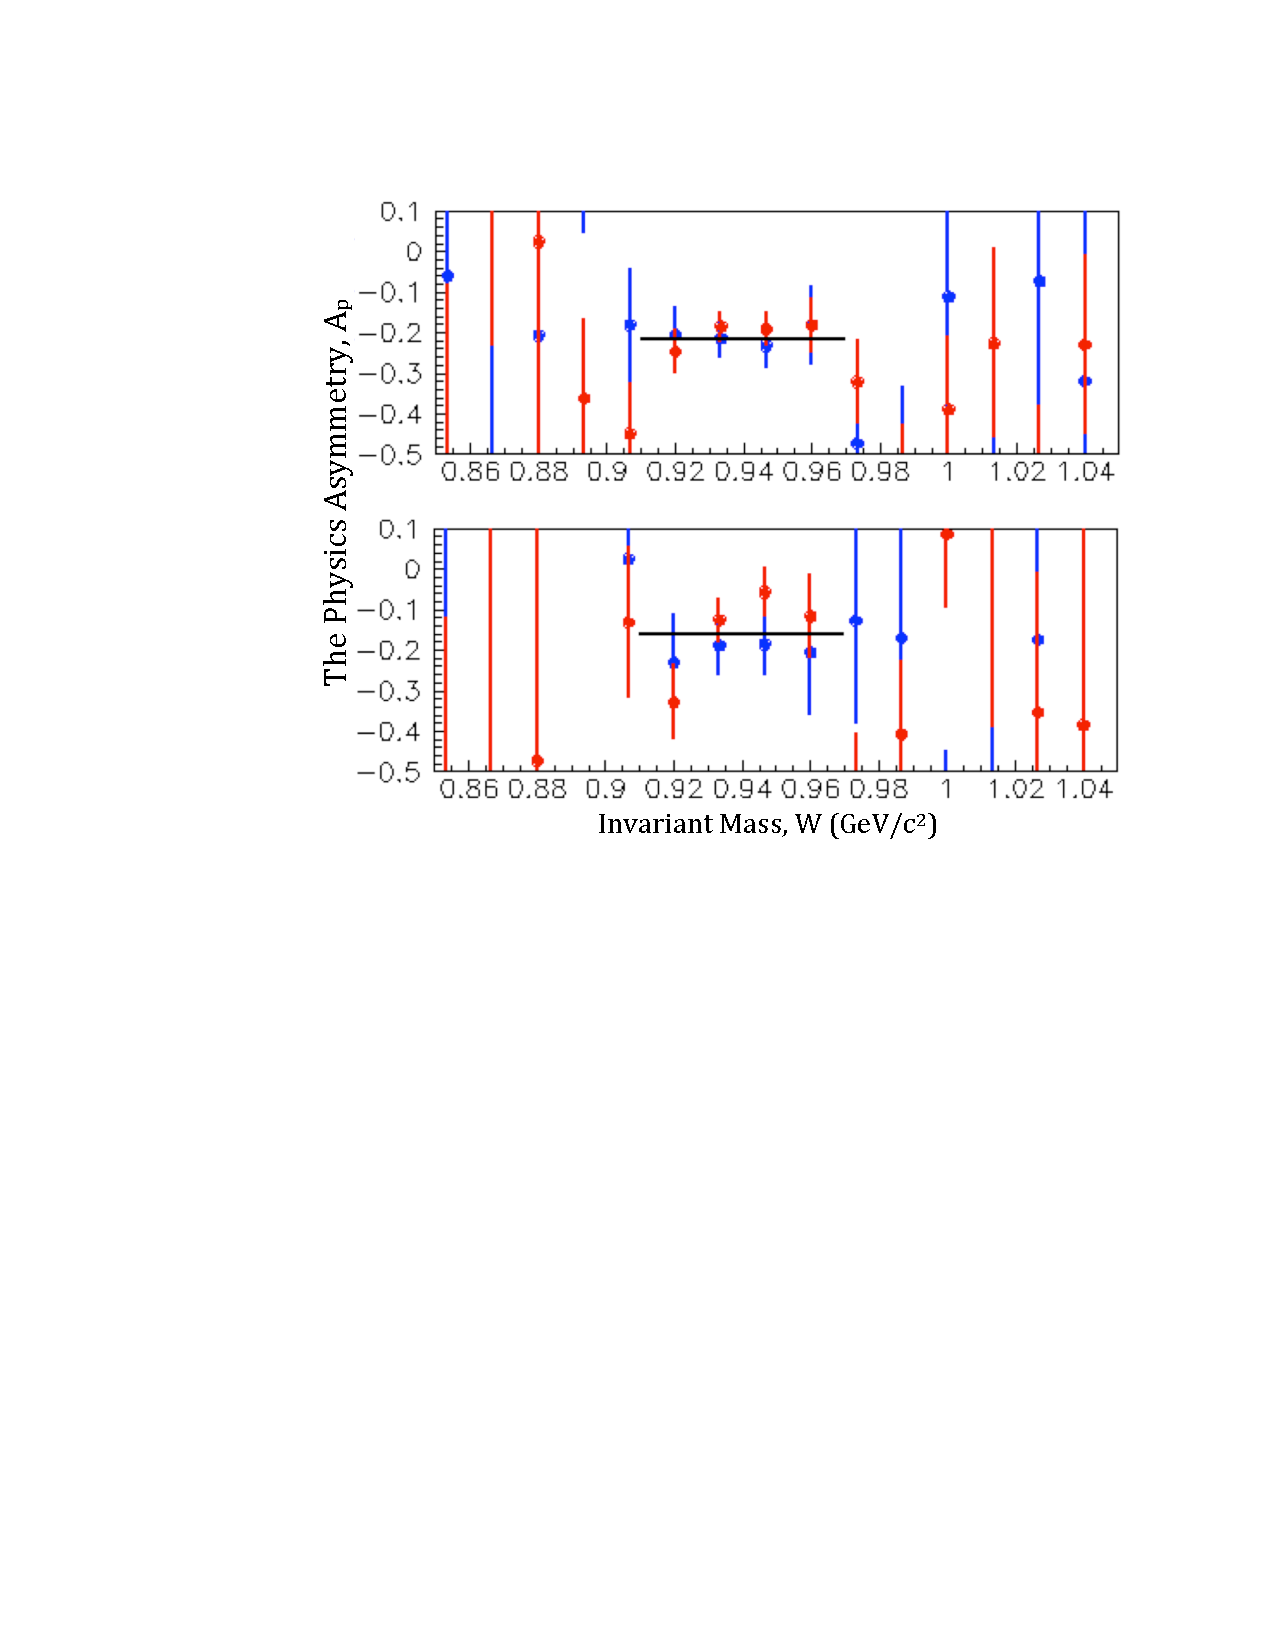
\includegraphics[width=\textwidth]{apsingle}
                \label{apsingled}
      \end{subfigure}
          \begin{subfigure}[htbp]{0.5\textwidth}
                \centering
               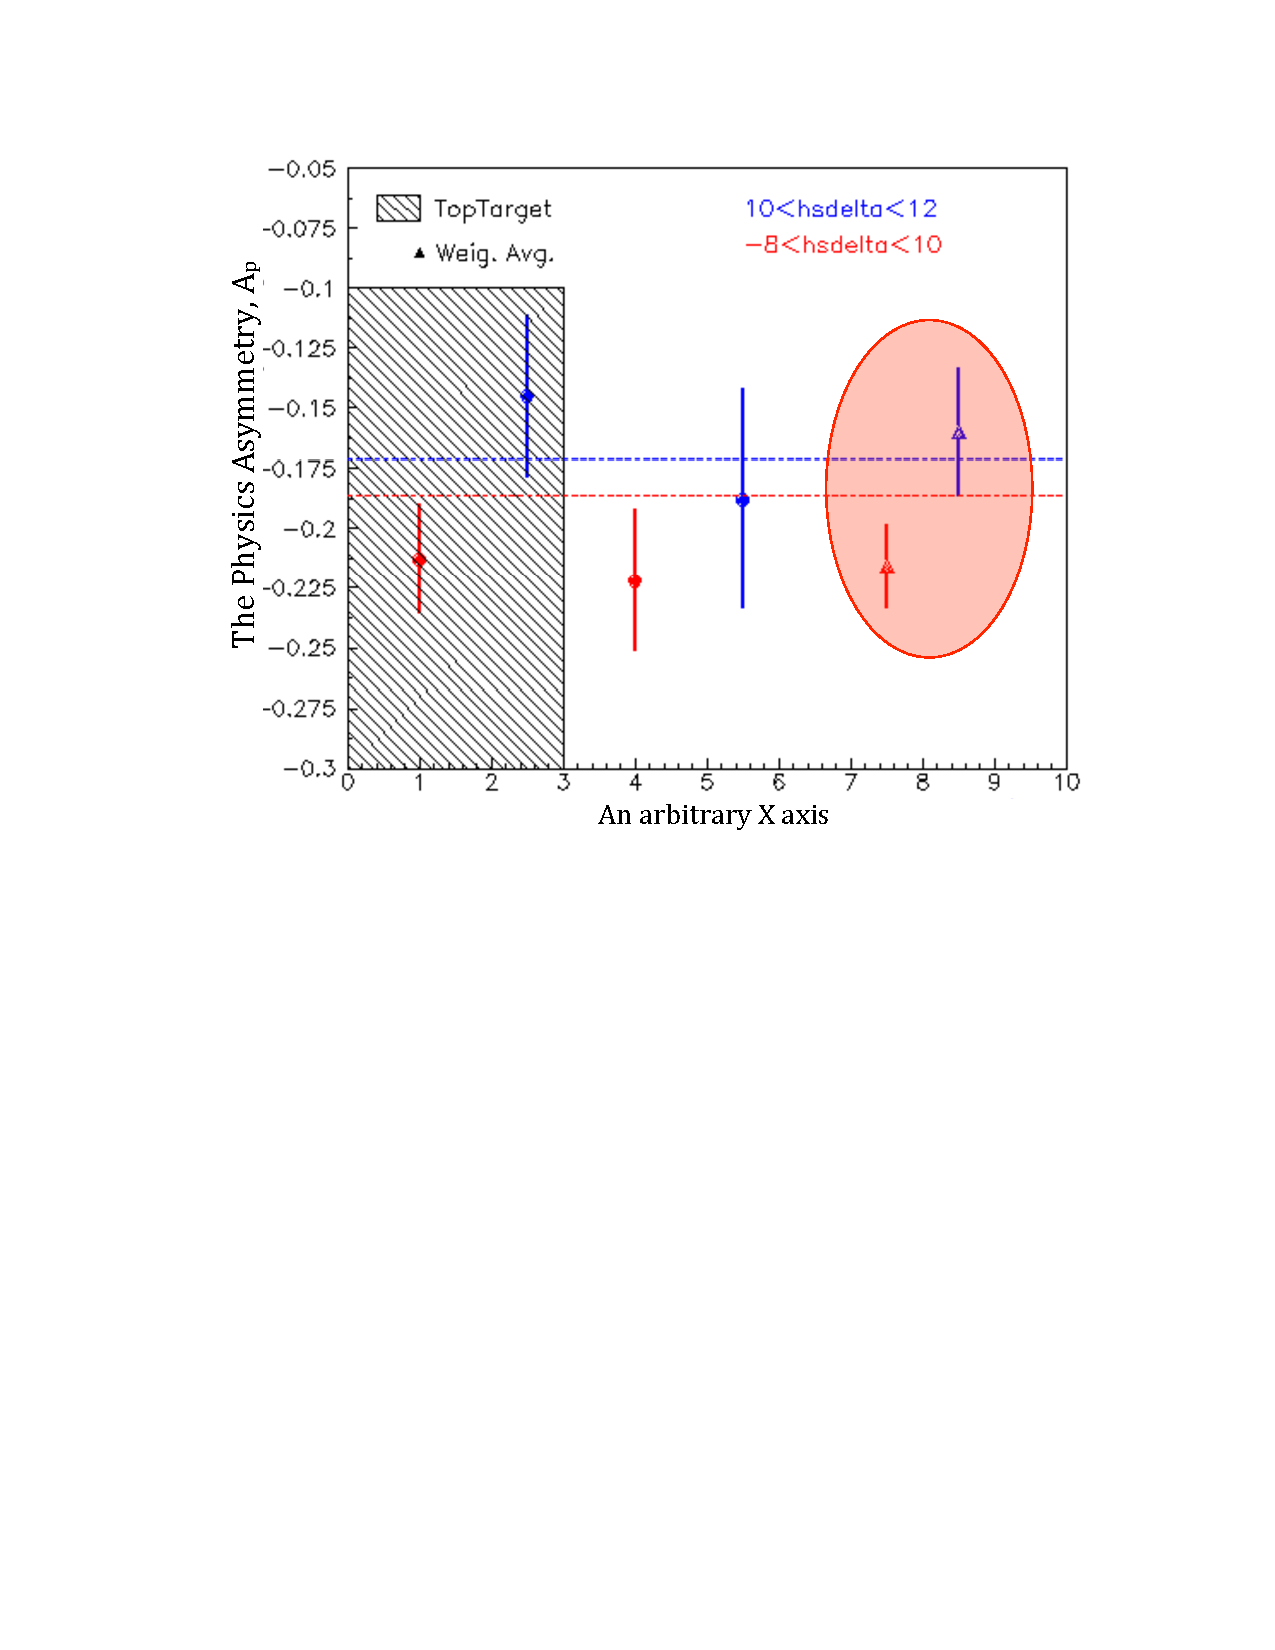
\includegraphics[width=\textwidth]{apsingletb}
                \label{apsingletb}
        \end{subfigure}    
\caption{(\emph{Left}): The top and bottom target physics asymmetries for the two different delta regions $-8\% \textless \delta \textless 10\%$ (\emph{top}) and $10\% \textless \delta \textless 12\%$ (\emph{bottom}). 
(\emph{Right}): The constant physics asymmetries for both top (inside the hatched box) and bottom (outside the hatched box) targets and the weighted average of it (inside the ellipse) for two different $\delta$ regions. The expected physics asymmetries from the known form factor ratio for each $Q^2$ by Kelly's form factor parametrization \cite{99} are also shown by dashed lines separately for the two different $\delta$ regions.}
\label{apsinglearm}                  
\end{figure}

The background shape under the elastic peak for the coincidence data was generated using the carbon target. The simulated carbon background was normalized by the scaling factor which was determined by the ratio of data-to-SIMC yields for the region of 0.03\textless$\delta p/p$\textless0.08 where the data and the simulated carbon background match each other. By adding this normalized carbon background to the SIMC-simulated H, a better match between the total data and SIMC-simulated H+C can be seen in Figure \ref{apcoin} (\emph{left}). Because the coincidence data were taken for two beam energies, 5.89 GeV and 4.73 GeV, this background simulation was done separately for both energies. The dilution factor was then calculated using Equation \eqref{dfsin}. Here, for the Equation \eqref{dfsin}, carbon was used instead of N+He+Al. Because of the low statistics, the average dilution factor was calculated using the integrals of both the normalized carbon MC and the measured counts under the elastic peak over the $\delta p/p$ region with a narrower cut of $\pm$0.02 instead of normalizing the raw asymmetry bin-by-bin with the dilution factor, f as a function of $\delta p/p$. The dilution factors calculated from the integration method for the top and bottom targets for the 5.895 GeV beam energy was determined as 0.785 and 0.830, respectively, while that for the 4.73 GeV beam energy was determined as 0.816.

To have better statistics from the low statistics coincidence data, all the coincidence runs were separated to a few categories at first as the data taken from top and bottom targets, positive and negative beam and target polarizations for each target cup, and so on. By normalizing $A_r/P_B/P_T$ with the calculated dilution factors, the physics asymmetries, $A_p$ were obtained for each category of the data set. Figure \ref{apcoin} (\emph{right}) shows the extracted physics asymmetries for different categories for both beam energies.

\begin{figure}[htbp]
\centering
        \begin{subfigure}[htbp]{0.46\textwidth}
               \centering
               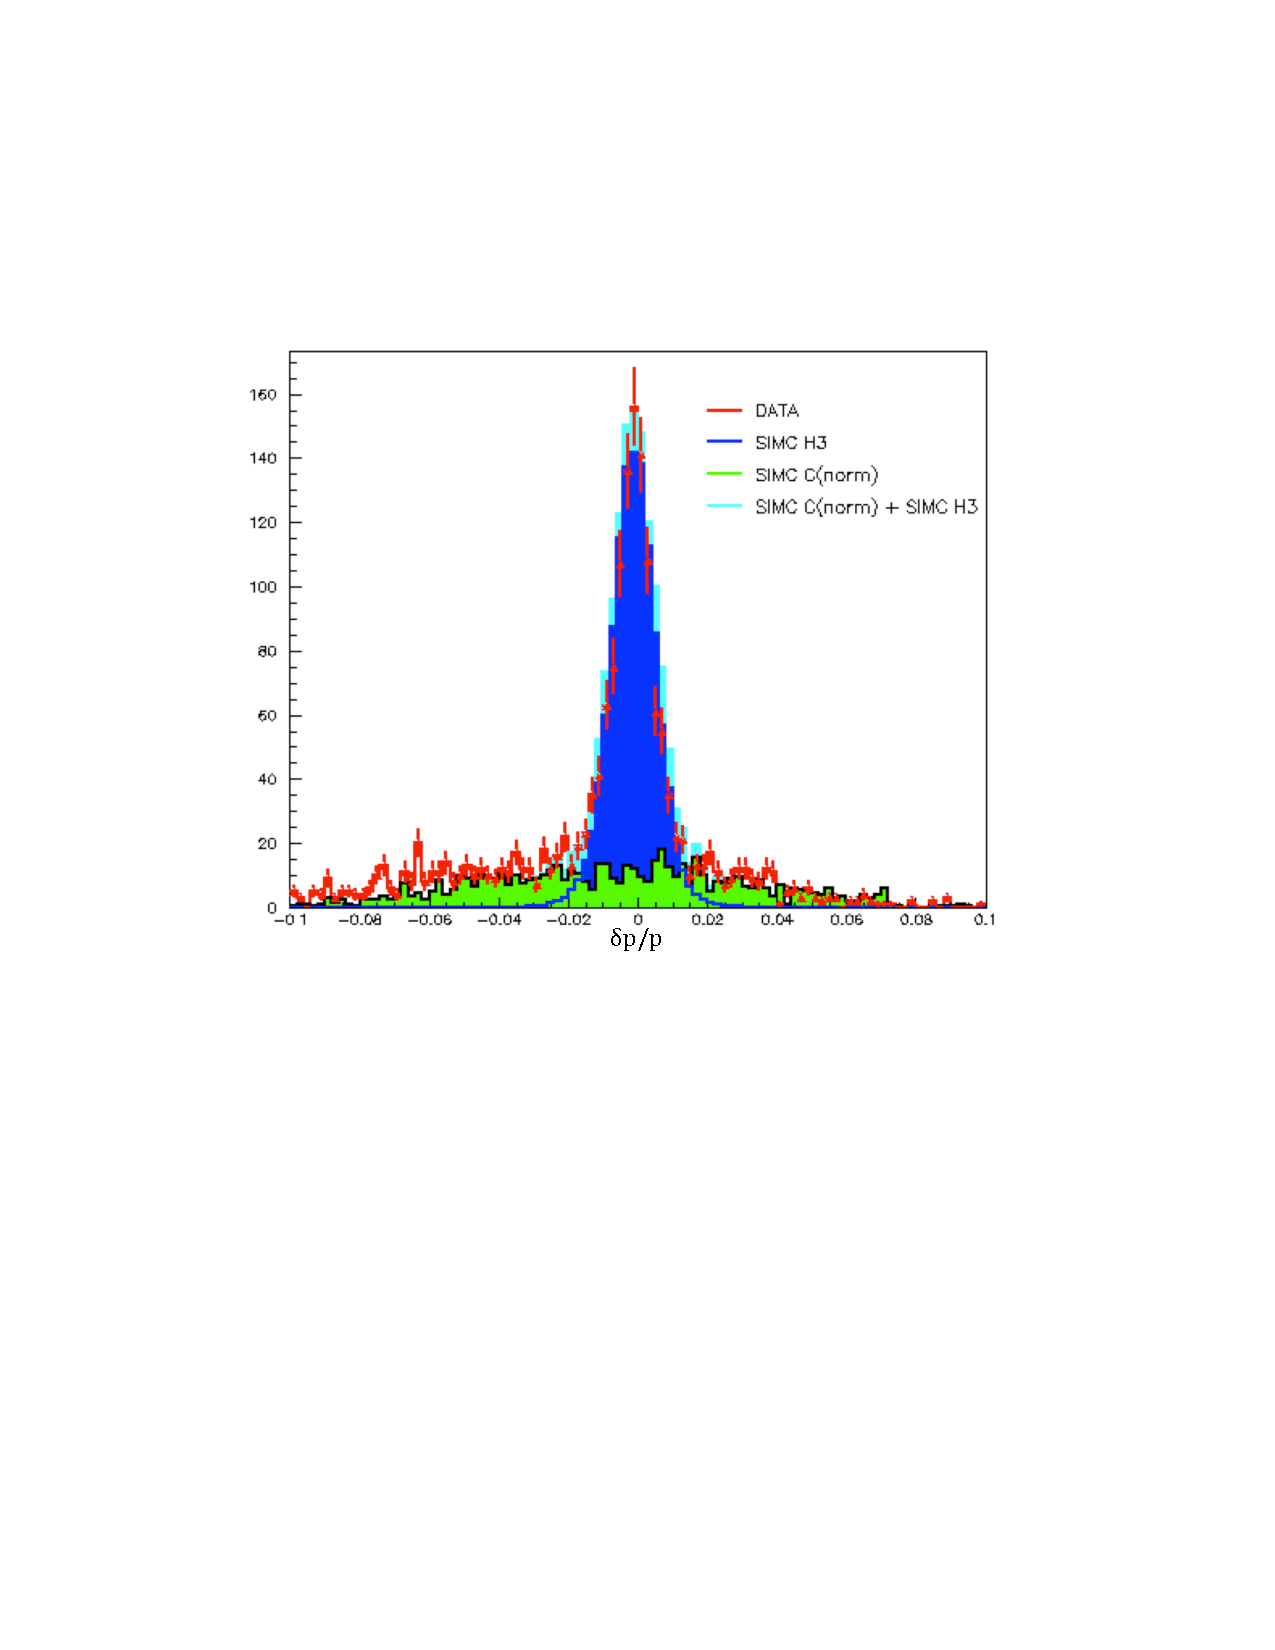
\includegraphics[width=\textwidth]{cnorm_5}
                \label{apsingled}
      \end{subfigure}
          \begin{subfigure}[htbp]{0.39\textwidth}
                \centering
               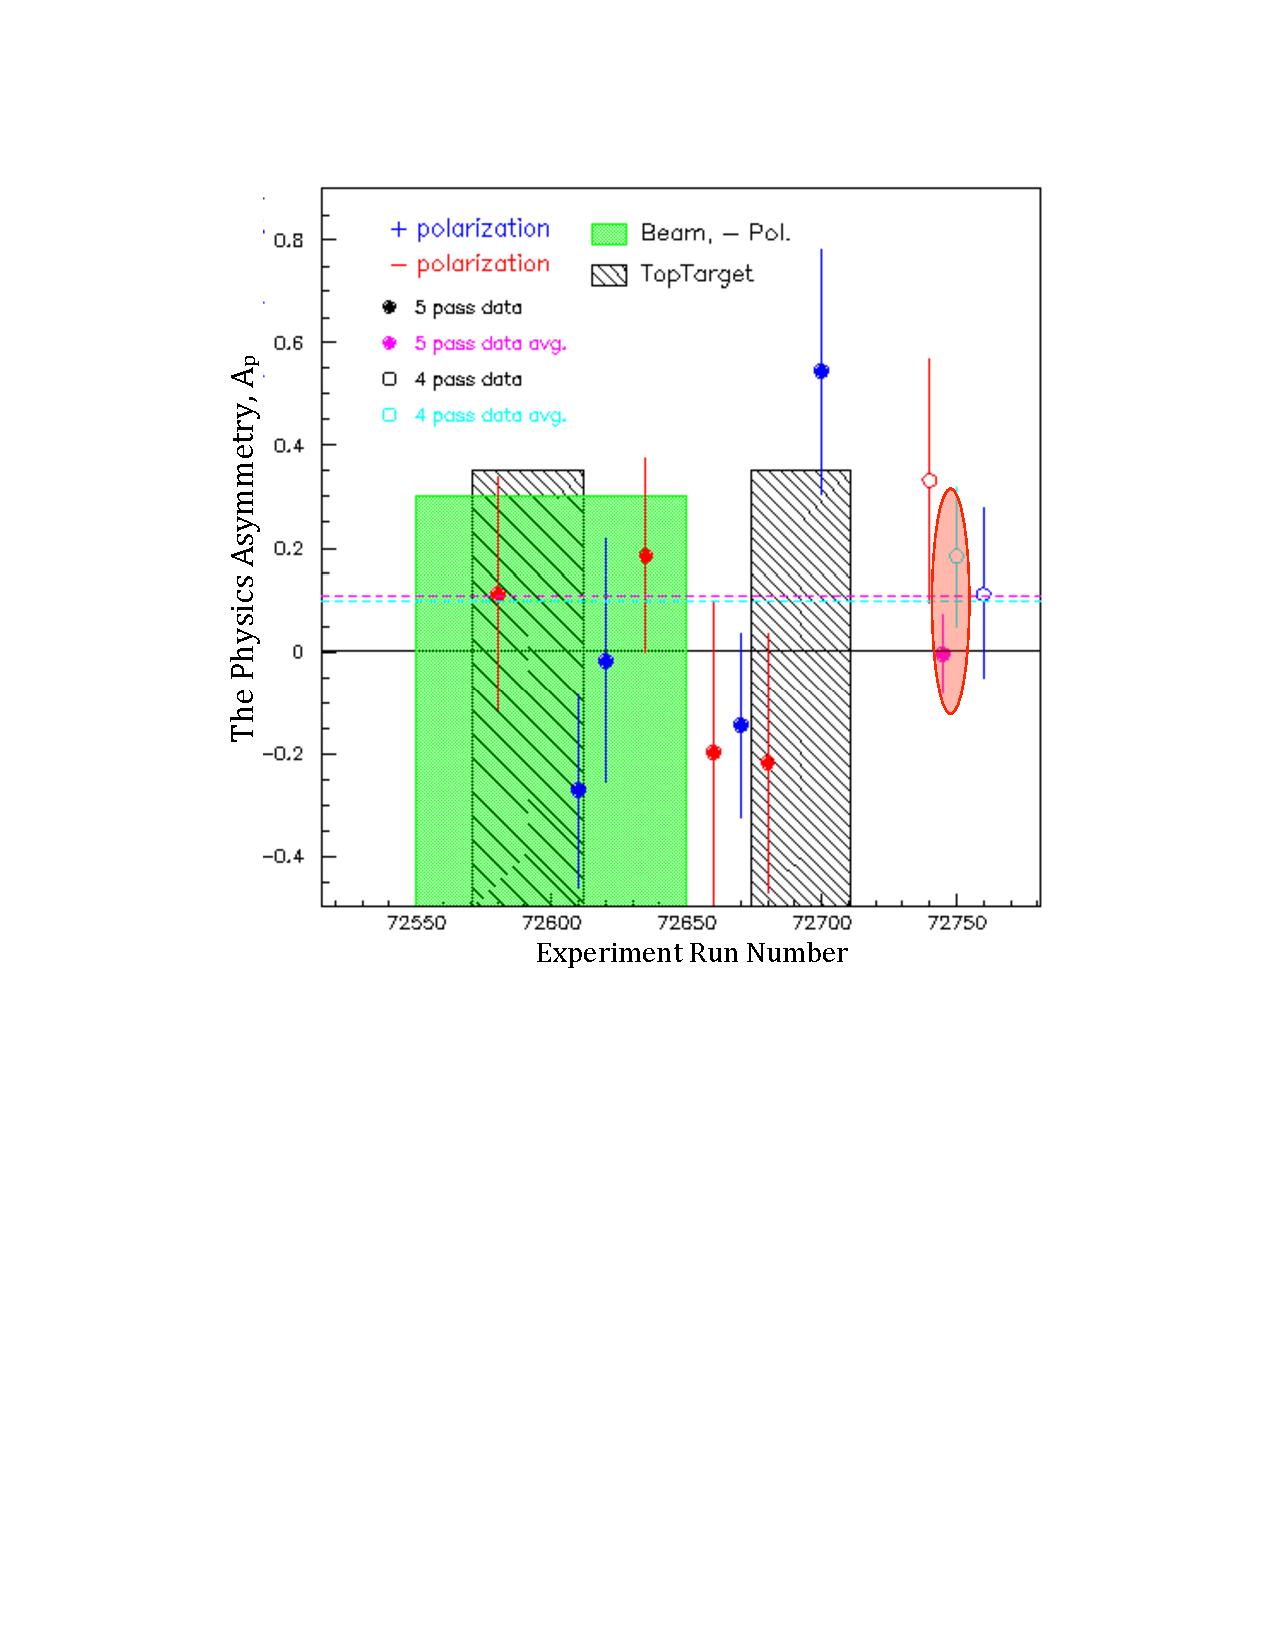
\includegraphics[width=\textwidth]{simc_ap}
                \label{apsingletb}
        \end{subfigure}    
\caption{\emph{Left}: The normalized carbon background (green) and $H$ (blue) comparison to the coincidence data (red) for the beam energy $5.89$ GeV. \emph{Right}: The physics asymmetries for each category of the coincidence data. The solid circles show the data from $5.895$ GeV beam energy and the empty circles show those from $4.73$ GeV beam energy. The $X$ axis shows an arbitrary run numbers. The weighted average physics asymmetries and their errors for the two beam energies are also shown (inside the brown ellipse). The dashed lines are the expected values of the physics asymmetries for the two beam energies $4.73$ GeV (light blue) and  $5.893$ GeV (magenta) calculated from the known form factor ratio for each $Q^2$ by Kelly's form factor parametrization \cite{99}.}
\label{apcoin}                  
\end{figure}

\vspace{0.3cm}
The weighted average physics asymmetries and their errors were calculated for the two beam energies as A=-0.006$\pm$0.077 for the beam energy 5.893 GeV, and A=0.184$\pm$0.136 for the beam energy 4.725 GeV. These results are also shown in the same Figure \ref{apcoin} (\emph{right}).

\vspace{0.3cm}
{
\raggedleft
\underline{\textbf{Extraction of $G^p_E/G^p_M$ Ratio}}
}


%The beam-target asymmetry, $A_p$ for elastic electron-proton scattering is directly related to the proton elastic form factor ratio, $G_E^p/G_M^p$ as;
% \begin{equation}
 %\begin{aligned}
%\label{btasym}
%A_p=\frac{-br\sin \theta^* \cos \phi^*-a\cos \theta^* }{r^2+c},
 %\end{aligned}
 %\end{equation}
%where $r=G_E^p/G_M^p$, and $\theta^*$ and $\phi ^*$ are the polar and azimuthal-angles between the momentum transfer vector, $\vec{q}$ and the proton's spin vector. The kinematic factors are given by,
 %\begin{equation}
 %\begin{aligned}
%\label{btasymabc}
%&a=2 \tau \tan \frac{\theta_e}{2}\sqrt{1+\tau+(1+\tau)^2\tan^2 \frac{\theta_e}{2}}\\
%&b=2 \tan \frac{\theta_e}{2}\sqrt{\tau(1+\tau)}\\
%&c=\tau+2\tau(1+\tau)\tan^2\frac{\theta_e}{2}
%\end{aligned}
 %\end{equation}
%with $\tau=\frac{Q^2}{4M^2}$. 

From the beam-target asymmetry Equation \eqref{btasym}, one can extract the $G_E^p/G_M^p$. The four-momentum transfer squared, $Q^2(E, E', \theta_e)$ for the elastic events were extracted from the data and compared with the Monte Carlo simulation yields. After applying all of the elastic event selection cuts on both data and the MC yields, the simulated background yields were subtracted from the data and the mean values of $Q^2$ were read from the resulting $Q^2$ distributions. The mean of the measured (calculated using elastic kinematics of the proton in HMS) electron scattering angle, $\theta_e$ was determined by applying all of the electron selection cuts on single-arm (coincidence) data. The polar and azimuthal angles, $\theta^*$ and $\phi ^*$ were calculated as,
 \begin{equation}
 \begin{aligned}
\label{thetastar}
&\theta^*=\arccos (-\sin \theta_q\cos\phi_e\sin\beta+\cos\theta_q\cos \beta)\\
&\phi^*=-\arctan\left(\frac{\sin \phi_e \sin \beta}{\cos \theta_q \cos \phi_e \sin \beta + \sin \theta_q \cos \beta}\right)+180^{\circ}.
\end{aligned}
\end{equation}

The out-of-plane angle of the scattered electron, $\phi_e$ was obtained by reading the mean value of the measured $\phi_e$ distribution for the elastic events. The three-momentum transfer vector, $\vec{q}$ points at an angle $\theta_q$, which is the scattered proton angle, determined (measured) event-by-event for the elastic kinematics of the electron (proton) in the HMS. The mean value of the $\theta_q$ distribution was obtained. The angle $\beta$ was the target magnetic field direction, 80$^{\circ}$ to the beam Z axis toward the BETA detector package. 

The Equation \eqref{btasym} has two solutions for $G_E^p/G_M^p$. The positive value was chosen because of the negative value is non physical. The error of the form factor ratio $G_E^p/G_M^p$, $\Delta r$ was determined by propagating the error from the physics asymmety, $\Delta A_p$.

The physics asymmetries $A_p$, and the extracted proton form factor ratios, $r=G_E^p/G_M^p$ together with the experimental parameters for both single-arm and coincidence data are shown in the Table \ref{tabasym}.
 \begin{table}[htbp]
   \centering
   \begin{tabular}{|l|c|c|c|c|} 
      \hline
         & \multicolumn{2}{c|}{single-arm} & \multicolumn{2}{c|}{Coincidence} \\
      \hline
         & $-8\% \textless \delta \textless 10\%$ & $10\% \textless \delta \textless 12\%$ & \multicolumn{2}{c|}{} \\
      \hline
      $E$            (GeV)                   & 5.895        & 5.895       &  5.893     &     4.725   \\
      $\theta_q$ (Deg)            &   44.38      &   46.50     &   22.23     &    22.60   \\
      $\phi_q$    (Deg)              & 171.80      & 172.20     & 188.40    &  190.90   \\      
      $\theta_e$ (Deg)            &   15.45      &   14.92     &    37.08    &     43.52  \\      
      $\phi_e$    (Deg)               & 351.80      & 352.10     &       8.40   &     10.95  \\
      $Q^2$ (GeV/c)$^2$           &      2.20      &      1.91    &       6.19   &        5.14  \\
      $\theta^*$ (Deg)            &     36.31    &    34.20    &  101.90   &     102.10 \\
      $\phi^*$ (Deg)                &   193.72    &  193.94    &       8.40   &       11.01 \\
      $A_p\pm \Delta A_p$         & $-0.205 \pm 0.018$ & $-0.139 \pm 0.026$ & $0.083 \pm 0.074$ & $0.248 \pm 0.138$\\
      $\mu_p r \pm \Delta (\mu_p r)$  & $0.576 \pm 0.217$  & $0.973 \pm 0.298$  & $0.439 \pm 0.411$   &  $-0.379\pm 0.690$\\
      \hline
      predicted $\mu_p r$               & $0.73$     & $0.78$      & $0.305$   &  $0.38$ \\
      predicted $A_p$                 & $-0.186$ & $-0.171$  & $0.107$   &  $0.097$\\
      \hline    
      \end{tabular}
   \caption{ The physics asymmetries and the extracted form factor ratios together with the experimental parameters  for both single-arm and coincidence data. The predicted ratio $\mu_p r$ from Kelly's form factor parametrization \cite{99} for each $Q^2$ and the calculated $A_p$ from the above predicted $\mu_p r$ are also shown. The errors $\Delta A_p$ and $\Delta(\mu_p r)$ are statistical.}
   \label{tabasym}
   \end{table}

\vspace{8 mm}

{
\raggedleft
\underline{\textbf{Systematic Error Estimation}}
}

The errors arising from the kinematic quantities were estimated by varying each quantity, one at a time by its corresponding uncertainty ($0.05$$\%$ for the beam energy, $0.1$$\%$ for the central momentum, and $0.5$ mrad for the spectrometer angle) and by propagating it to the Monte Carlo extracted $G_E^p/G_M^p$ ratio. The resulting difference between the extracted $G_E^p/G_M^p$ ratio from the value at the nominal kinematics and the value with the kinematic uncertainty was taken as the uncertainty in the $G_E^p/G_M^p$ ratio due to the uncertainty in that quantity. In general, the uncertainties due to the kinematic variables were less than $1$$\%$. 

Using the Jacobian of the elastic electron-proton reaction, the error on the  $ \theta_q$, $\delta \theta_q$ were obtained from the beam energy E and the scattered electron angle $\theta_e$ which was estimated as 0.03$^{\circ}$. Further, using the uncertainty of the target magnetic field direction, $\beta$, $\delta \beta=0.1^{\circ}$, the uncertainties of  $\theta^*$ and $\phi ^*$ were estimated. The error of the $G_E^p/G_M^p$ from the error of the $\theta^*$ was estimated as 0.54\%, while that from the $\phi ^*$ was estimated as 0.01\%.

The accuracy of the target polarization was based on the accuracy of the calibration constants used to produce the absolute polarization from the NMR area. The systematic error on the target polarization was estimated as 5\% \cite{109}. The error of the beam polarization measurement comes from a global error of the M$\phi$ller measurements and the error due to the fit to these measurements. The beam polarization uncertainty during SANE was measured as 1.5\% \cite{109}.

For both single-arm and coincidence data sets, the dilution factors have been determined using data-to-Monte Carlo simulated yield comparisons. Therefore, the uncertainty of the dilution factor was based on how well the data match with the simulated yields. Since the simulated yields were based on the packing fraction, the error of 5\% of the packing fraction measurement was propagated to the dilution factor. Therefore, the uncertainty of the form factor ratio, $G_E^p/G_M^p$ was determined as 1.34\%.

Single-arm data was using the extended momentum acceptance in the region of  $10\% \textless \delta \textless 12\%$, where the HMS optics were not well tested. Therefore, the reconstruction of the particle tracks from this region was not understood well. Therefore, the uncertainty of the COSY model was a special source of systematic uncertainty for the single-arm data. This has being  tested with the Monte Carlo simulation. The biggest loss of events in this higher $\delta$ region, $10\% \textless \delta \textless 12\%$ was identified as at the HMS vacuum pipe exit. The uncertainty due to this higher momentum electron tracks hitting the edge of the vacuum pipe exit was determined by applying $\pm$2 mm offsets on the vacuum pipe positions on both vertical and horizontal directions separately, and taking the effective solid angle differences between the offsets and those at the nominal vacuum pipe position. Taking the average ratio of these effective solid-angle differences to the nominal solid-angle, the uncertainty due to the particle track reconstruction was estimated as 0.68\%. However, during the dilution factor determination, Monte Carlo simulated C cross-section shape match was done for the data in the both $\delta$ regions. Also, Monte Carlo yields were normalized with the ratio of data-to-Monte Carlo yields in the region of 0.7\textless W \textless 0.85 GeV/c$^2$. Therefore, the uncertainty, 0.68\% that comes from losing events due to higher $\delta$ were already accounted in the dilution factors.

Table \ref{tabsys} summarizes non-negligible contributions to the systematic uncertainty of the single-arm data. The measurements, the uncertainty of each measurement and the relative systematic uncertainty of the  $\mu_p G_E^p/G_M^p$ ratio due to the uncertainty on that measurement are shown. The final relative systematic uncertainty was obtained by summing all the individual contributions quadratically. Summing all the individual contributions of the systematic uncertainties linearly represents the maximum possible error of the measurement. Therefore, the final relative systematic error on $\mu_p G_E^p/G_M^p$ was estimated as $5.44$$\%$ while the maximum possible error was estimated as $9.13$$\%$. The target, beam polarizations and the packing fraction were the dominant contributions to the systematic uncertainty.
\\~
  \begin{table}[htbp]
   \centering
   \begin{tabular}{|l|c|c|} 
      \hline
         Measurement              & Error                                                 & $\Delta \mu_p G_E^p/G_M^p / \mu_p G_E^p/G_M^p$ $(\%)$  \\
      \hline
      $E$ (GeV)             &  $0.003$                             &   0.07   \\
      $E'$ (GeV)                 &  $0.004$                              &    0.13   \\      
      $\theta_e$ (mrad)      &   0.5                                    &    0.54   \\          
      $\theta^*$ (mrad)       &   1.22                                                         &    0.54          \\
      $\phi^*$ (mrad)          &    0.3                                                        &     0.01         \\      
      $P_T$   ($\%$)                          &  5.0                                           &    5.0    \\
      $P_B$     ($\%$)                        & 1.5                                            &   1.5     \\
      Packing Fraction, \emph{pf}   ($\%$)                                 &  5 &   1.34   \\
%      $10 \textless \delta \textless 12$   &         0.68 $\%$             &              \\            
      \hline
      \multicolumn{2}{|l|}{The maximum possible error}                                                          &   9.13    \\
      \hline
      \multicolumn{2}{|l|}{The final error}                                                          &   5.44    \\
      \hline      
  \end{tabular}
   \caption{ The systematic uncertainty on each measurement and the relative systematic uncertainty on the $\mu_p G_E^p/G_M^p$ ratio due to the uncertainty on that measurement for the single-arm data. The maximum possible systematic uncertainty and the final systematic uncertainty  are also shown.}
   \label{tabsys}
   \end{table}

{
\raggedleft
\underline{\textbf{Results and the discussion}}
}

The results for the proton elastic form factor ratio, $\mu_p G_E^p/G_M^p$, determined for both data sets, single-arm and coincidence, are shown in Table \ref{tabasym}. The resulting form factor ratio from the two regions of the HMS momentum acceptance was determined by extrapolating both measurements to the average $Q^2$ using Kelly's parametrization \cite{99} and then taking the weighted average of the two form factor ratios. The resulting form factor ratio, $\mu_p G_E^p/G_M^p=0.720\pm0.176\pm0.039$ was obtained for an average four-momentum transfer squared $Q^2=2.06$ (GeV/c)$^2$.

Due to the low statistics of the coincidence data, the form factor ratios at the two beam energy settings were also decided to combine. The weighted average $\mu_p G_E^p/G_M^p$ and its error were obtained from the two measurements which were extrapolated to the average $Q^2$ using Kelly's parametrization \cite{99}. Because of the larger statistical error of the coincidence data point at the average $Q^2=5.66$ (GeV/c)$^2$, the systematic uncertainty was estimated based on the detailed systematics study at the low $Q^2$ point and found negligible.

Therefore the resulting form factor ratio and it's error were obtained as $\mu_p G_E^p/G_M^p=0.244\pm0.353\pm0.013$ for an average $Q^2=5.66$ (GeV/c)$^2$.

Table \ref{final} shows the final $\mu_p G_E^p/G_M^p$ ratios together with the statistical and systematic uncertainties for each  average $Q^2$ values.  
%\\~
%\vspace{-0.1cm}
  \begin{table}[htbp]
   \centering
   \begin{tabular}{|l|c|} 
      \hline
      $Q^2_{Avg}$ (GeV/c)$^2$     & $\mu_p G_E^p/G_M^p \pm \Delta \mu_p G_E^p/G_{M(stat)}^p \pm \Delta \mu_p G_E^p/G_{M(syst)}^p$\\
      \hline
      $2.06$                            &  0.720 $\pm$ 0.176 $\pm $ 0.039  \\
      $5.66$                            &  0.244 $\pm$ 0.353  $\pm $ 0.013  \\     
      \hline
  \end{tabular}
     \vspace{-0.1cm}
   \caption{The results of the form factor analysis from the experiment SANE.}
   \label{final}
   \end{table}

\vspace{-0.1cm}
Figure \ref{resultratio} shows the form factor measurements from SANE together with the world data as a function of $Q^2$. The inner-error bar is  systematic and the outer-error bar is statistical. 
\begin{figure}[htbp]
\centering
\mbox{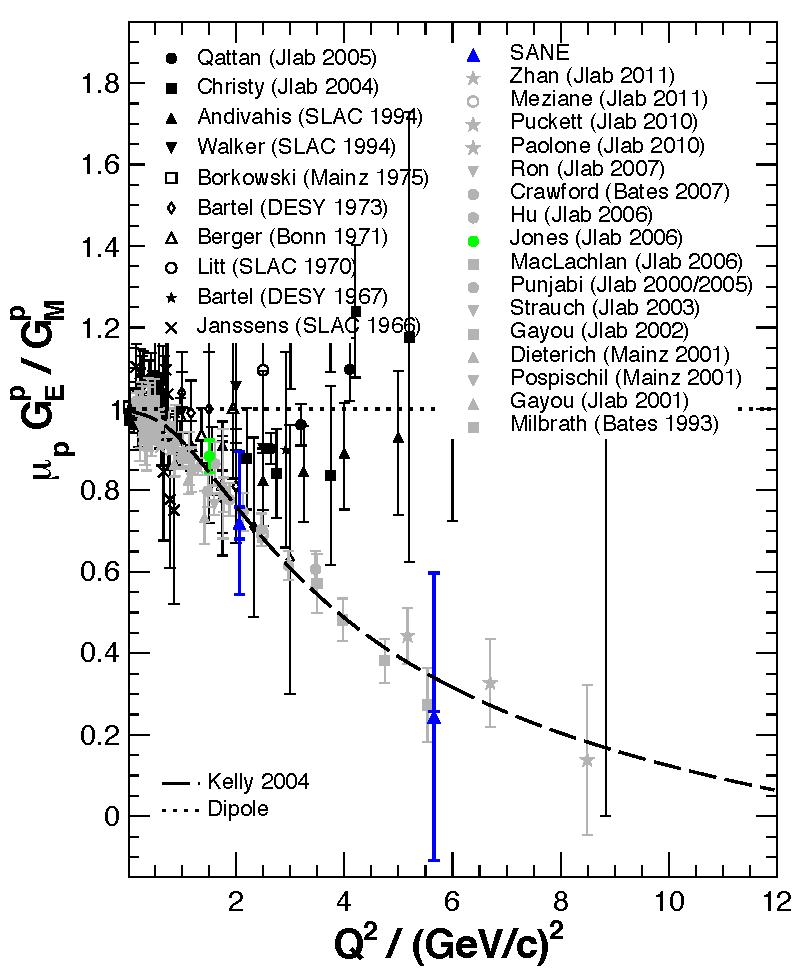
\includegraphics[scale=0.6]{ratio_final}}
\caption{The form factor measurements from SANE together with the world data as a function of $Q^2$. The inner-error bar is  systematic and the outer-error bar is statistical.}
\label{resultratio}
\end{figure}
The weighted average data points at $Q^2=2.06$ (GeV/c)$^2$ and $Q^2=5.66$ (GeV/c)$^2$ are very consistent with the existing recoil-polarization measurements, confirming the decrease of $\mu_p G_E^p/G_M^p$ with $Q^2$. Because theoretically, the beam-target asymmetry method is equivalent to the polarization-transfer method, the results were expected to be similar to the polarization-transfer data. The measurement did not revealed any unknown systematic difference from the polarization-transfer method. The obtained accuracy confirms the suitability of using the beam-target asymmetry for determination of  the $\mu_p G_E^p/G_M^p$ ratio. 

The weighted average data point at higher  $Q^2=5.66$ (GeV/c)$^2$ has a larger statistical uncertainty due to the small number of counts.
% which makes it difficult to draw a strong conclusion with respect to a change of the proton form factor ratio with $Q^2$. 
The HMS drift chamber gas leak during the coincidence data taking was resulted about $\sim$60 \% inefficiency of the elastic proton detection by the HMS. In addition to that, due to a damage of the superconducting Helmholtz coils which used to polarize the NH$_3$ target, the production data-taking time was reduced. 
Therefore,  single-arm data were taken only about $\sim$12 hours in total and the coincidence data for elastic kinematics were taken about a week for both beam energies, $\sim$40 hours and $\sim$155 hours, respectively, for the two beam energies 4.72 GeV and 5.89 GeV. 
Along with optimum proton detection efficiency in HMS, it should be possible to take at least four times the amount of data in the same time period, which would decrease the error bars on both measurements by a factor of two. In addition, the target spin orientation were not optimized for the measurement of $G_E/G_M$.

{
\raggedleft
\underline{\textbf{Theoretical Interpretation}}
}

The experimental understanding of the proton form factors led to many theoretical attempts to explain the nucleon form factors. Despite their approximations and limitations, some of these non-perturbative methods reveal some insight into the nucleon structure. 

In non-relativistic approximation, $G_E$ and $G_M$ are the Fourier transforms of the charge and magnetic moment densities of the nucleon in the Breit frame. 
%However, only at $Q^2=0$, the Breit frame coincides with the lab frame and the form factor interpretation to the charge and magnetic moment distribution become valid. 
Kelly \cite{99} has derived a theoretical model relating the Sachs form factors to the rest frame charge and magnetic moment densities taking relativity into account. However, this is strictly model-dependent since the Lorentz boost for a composite object such as proton depends on the interactions among the constituent quarks. The most important feature of the proton density from this model is the broader shape of the charge density relative to the magnetic moment density, reflecting the precise recoil-polarization data in which $G_E^p$ falls faster than $G_M^p$ at large $Q^2$. 

The earliest model, Vector Meson Dominance (VMD) explained the dipole behavior of the nucleon form factors. In this model, the photon couples to the nucleon through the exchange of the three lightest vector mesons, $\rho$ (770), $\omega$ (782) and $\phi$ (1020). In elastic electron-nucleon scattering, the form factors at low $Q^2$ are dominated by these vector mesons. The first VMD fit was performed by Iachello \emph{et al.} \cite{111} and a linear decrease of the proton $\mu_p G_E^p/G_M^p$ ratio has been predicted for $Q^2\textgreater1$ (GeV/c)$^2$, which is an agreement with the result from the polarization-transfer technique. Gari and Krumpelmann \cite{112} extended the model to conform with pQCD scaling at larger $Q^2$ with a smooth transition from VMD picture hold at low $Q^2$. Thereafter, many extended VMD fits have been obtained which provided a good parameterization of  nucleon electromagnetic form factors \cite{113, 114, 115, 116}.

Constituent Quark Models (CQM) were developed to understand the structure of the nucleons in terms of quark and gluon degrees of freedom. The Isgur-Karl model \cite{117} is an example, in which the quarks are confined by a long-range harmonic oscillator potential supplemented by a short-range one-gluon-exchange quark-quark interaction. Since the quarks are much lighter than the nucleon; they need to be treated relativistically following the prescriptions by Dirac \cite{118}, which describes the form factor behavior at large $Q^2$. However, a pion cloud and a finite size of the constituent quarks were introduced to this model to correctly describe the behavior at lower $Q^2$. Miller \cite{119} added the effects of the pion cloud of the nucleon to the relativistic constituent quark model (rCQM) of the Light-Front Cloudy Bag Model \cite{120} which involves relativistic pion-nucleon form factors. The pion cloud effects within this model made large contributions at low $Q^2$, particularly for the neutron electric form factor, which is not well reproduced by the rCQM alone. In contrast, quarks are found to dominate at large $Q^2$. 

At higher $Q^2$, quarks and gluons play a dominant role in the form factors in which the perturbative QCD (pQCD) makes a prediction about the behavior of these. The constancy of the Rosenbluth data for $\mu_p G_E^p/G_M^p$ was consisted with the pQCD dimensional scaling laws \cite{121}, valid for asymptotically large $Q^2$. These predictions are different from the polarization-transfer measurements, where the ratio $R=\mu_p G_E^p/G_M^p$ shows roughly a linear decrease with $Q^2$ and points toward a zero-crossing at some larger $Q^2$. The decrease of $R$ with $Q^2$ was later interpreted in pQCD by Belitsky \emph{et al.} \cite{122} introducing the quark orbital angular momentum. The recoil-polarization data for $F_2^p/F_1^p$ are compatible with such a scaling for the entire $Q^2$ range of the data.

Generalized Parton Distributions (GPDs) are the theoretical framework to understand the quark structure of the nucleon. The predictions for the nucleon form factors are derived using a model for the GPDs by Guidal \emph{et al.} \cite{123}, which achieves a very good agreement with experimental data for all four nucleon form factors in the entire $Q^2$ range. Because GPDs can be related to the total angular momentum carried by the quark in the nucleon, it allows an evaluation of Ji's angular momentum sum rules \cite{124}. Furthermore, the vector GPDs have been used to derive model-independent representations of the nucleon transverse charge and magnetization densities as two-dimensional Fourier transforms of the Dirac ($F_1$) and Pauli ($F_2$) form factors \cite{125}.

A complementary framework for studying the form factors is via Dyson-Schwinger Equations (DSEs) \cite{126, 127}. The investigation of hadron structure in the Dyson-Schwinger approach proceeds for baryons via the covariant Faddeev Equation \cite{128, 129}. This approach provides access to all momentum scales and all quark masses, which is in good agreement in form factor results with the experimental data above $Q^2\simeq2$ (GeV/c)$^2$. This has been shown that the orbital angular momentum contributes one-third to the nucleon spin, and this contribution slowly decrease with rising current quark mass.

 Quark-diquark model studies also found a zero-crossing, where its location depends on the model parameters in the calculation \cite{130, 131}. The overall agreement between the \cite{129} and those obtained in the quark-diquark model provides further evidence for the quark-diquark structure of the nucleon.

Lattice gauge theory can provide an \emph{ab initio} calculation in contrast to the all of the other models which have constructed to focuss on selected aspects of QCD. One of the most advanced lattice calculations of electromagnetic form factors has been performed by the QCDSF collaboration \cite{132}. Ashley \emph{et al.} \cite{133} have extrapolated the results of these calculations appropriate to full QCD. Lattice QCD results from LHPC Collaboration \cite{134} performed for the nucleon electromagnetic form factors shows that the Dirac isovector form factor $F_1^V$ in qualitative agreement with data and the isovector ratio $F_2^V/F_1^V$ approaches the experimental results when decreasing $m_{\phi}$ from 360 MeV. An extensive discussion of the theoretical model explanation on the form factors can be found in the review paper \cite{135}.




{
\raggedleft
\underline{\textbf{Conclusion}}
}

Measurement of the beam-target asymmetry in elastic electron-proton scattering offers an independent technique of determining the proton elastic form factor ratio, $\mu_p G_E^p/G_M^p$. The TPE amplitude has a strong $\epsilon$ dependence with a large effect on the extraction of the proton form factors from the Rosenbluth separation method. The absence of such a strong dependence for the polarizable observables, the double-spin polarization experiments show a strong validation of the method of measuring the form factor ratio.

 The form factor analysis from the experiment SANE extended the proton electric-to-magnetic form factor ratio, $\mu_p G_E^p/G_M^p$ from the double-spin asymmetry up to $Q^2=5.66$ (GeV/c)$^2$. The results at $Q^2=2.06$ (GeV/c)$^2$ are an important test of the reproducibility of the first measurement of the beam-target asymmetry at $Q^2=1.5$ (GeV/c)$^2$ \cite{60}. A measurement with this method at higher $Q^2$ than the first measurement at $Q^2=1.5$ (GeV/c)$^2$ has been very important to see if this third technique is consistent with the polarization-transfer method as expected, or if it follows the form factor scaling result from the Rosenbluth separation method. The result of this work validates those of the polarization-transfer method and, therefore, strengthens the case for the TPE framework as an explanation for the form factor discrepancy between unpolarized and polarized data.

However, as a byproduct measurement of the SANE experiment, the precision of this result is limited by statistics. It would certainly be possible to improve the precision at high $Q^2$ with a dedicated experiment. 

\clearpage
\singlespacing
\bibliographystyle{unsrt}
\bibliography{ref}

\end{document} 


